\documentclass[conference, fleqn]{IEEEtran}

%% ODER: format ==         = "\mathrel{==}"
%% ODER: format /=         = "\neq "
%
%
\makeatletter
\@ifundefined{lhs2tex.lhs2tex.sty.read}%
  {\@namedef{lhs2tex.lhs2tex.sty.read}{}%
   \newcommand\SkipToFmtEnd{}%
   \newcommand\EndFmtInput{}%
   \long\def\SkipToFmtEnd#1\EndFmtInput{}%
  }\SkipToFmtEnd

\newcommand\ReadOnlyOnce[1]{\@ifundefined{#1}{\@namedef{#1}{}}\SkipToFmtEnd}
\usepackage{amstext}
\usepackage{amssymb}
\usepackage{stmaryrd}
\DeclareFontFamily{OT1}{cmtex}{}
\DeclareFontShape{OT1}{cmtex}{m}{n}
  {<5><6><7><8>cmtex8
   <9>cmtex9
   <10><10.95><12><14.4><17.28><20.74><24.88>cmtex10}{}
\DeclareFontShape{OT1}{cmtex}{m}{it}
  {<-> ssub * cmtt/m/it}{}
\newcommand{\texfamily}{\fontfamily{cmtex}\selectfont}
\DeclareFontShape{OT1}{cmtt}{bx}{n}
  {<5><6><7><8>cmtt8
   <9>cmbtt9
   <10><10.95><12><14.4><17.28><20.74><24.88>cmbtt10}{}
\DeclareFontShape{OT1}{cmtex}{bx}{n}
  {<-> ssub * cmtt/bx/n}{}
\newcommand{\tex}[1]{\text{\texfamily#1}}	% NEU

\newcommand{\Sp}{\hskip.33334em\relax}


\newcommand{\Conid}[1]{\mathit{#1}}
\newcommand{\Varid}[1]{\mathit{#1}}
\newcommand{\anonymous}{\kern0.06em \vbox{\hrule\@width.5em}}
\newcommand{\plus}{\mathbin{+\!\!\!+}}
\newcommand{\bind}{\mathbin{>\!\!\!>\mkern-6.7mu=}}
\newcommand{\rbind}{\mathbin{=\mkern-6.7mu<\!\!\!<}}% suggested by Neil Mitchell
\newcommand{\sequ}{\mathbin{>\!\!\!>}}
\renewcommand{\leq}{\leqslant}
\renewcommand{\geq}{\geqslant}
\usepackage{polytable}

%mathindent has to be defined
\@ifundefined{mathindent}%
  {\newdimen\mathindent\mathindent\leftmargini}%
  {}%

\def\resethooks{%
  \global\let\SaveRestoreHook\empty
  \global\let\ColumnHook\empty}
\newcommand*{\savecolumns}[1][default]%
  {\g@addto@macro\SaveRestoreHook{\savecolumns[#1]}}
\newcommand*{\restorecolumns}[1][default]%
  {\g@addto@macro\SaveRestoreHook{\restorecolumns[#1]}}
\newcommand*{\aligncolumn}[2]%
  {\g@addto@macro\ColumnHook{\column{#1}{#2}}}

\resethooks

\newcommand{\onelinecommentchars}{\quad-{}- }
\newcommand{\commentbeginchars}{\enskip\{-}
\newcommand{\commentendchars}{-\}\enskip}

\newcommand{\visiblecomments}{%
  \let\onelinecomment=\onelinecommentchars
  \let\commentbegin=\commentbeginchars
  \let\commentend=\commentendchars}

\newcommand{\invisiblecomments}{%
  \let\onelinecomment=\empty
  \let\commentbegin=\empty
  \let\commentend=\empty}

\visiblecomments

\newlength{\blanklineskip}
\setlength{\blanklineskip}{0.66084ex}

\newcommand{\hsindent}[1]{\quad}% default is fixed indentation
\let\hspre\empty
\let\hspost\empty
\newcommand{\NB}{\textbf{NB}}
\newcommand{\Todo}[1]{$\langle$\textbf{To do:}~#1$\rangle$}

\EndFmtInput
\makeatother
%
%
%
%
%
%
% This package provides two environments suitable to take the place
% of hscode, called "plainhscode" and "arrayhscode". 
%
% The plain environment surrounds each code block by vertical space,
% and it uses \abovedisplayskip and \belowdisplayskip to get spacing
% similar to formulas. Note that if these dimensions are changed,
% the spacing around displayed math formulas changes as well.
% All code is indented using \leftskip.
%
% Changed 19.08.2004 to reflect changes in colorcode. Should work with
% CodeGroup.sty.
%
\ReadOnlyOnce{polycode.fmt}%
\makeatletter

\newcommand{\hsnewpar}[1]%
  {{\parskip=0pt\parindent=0pt\par\vskip #1\noindent}}

% can be used, for instance, to redefine the code size, by setting the
% command to \small or something alike
\newcommand{\hscodestyle}{}

% The command \sethscode can be used to switch the code formatting
% behaviour by mapping the hscode environment in the subst directive
% to a new LaTeX environment.

\newcommand{\sethscode}[1]%
  {\expandafter\let\expandafter\hscode\csname #1\endcsname
   \expandafter\let\expandafter\endhscode\csname end#1\endcsname}

% "compatibility" mode restores the non-polycode.fmt layout.

\newenvironment{compathscode}%
  {\par\noindent
   \advance\leftskip\mathindent
   \hscodestyle
   \let\\=\@normalcr
   \let\hspre\(\let\hspost\)%
   \pboxed}%
  {\endpboxed\)%
   \par\noindent
   \ignorespacesafterend}

\newcommand{\compaths}{\sethscode{compathscode}}

% "plain" mode is the proposed default.
% It should now work with \centering.
% This required some changes. The old version
% is still available for reference as oldplainhscode.

\newenvironment{plainhscode}%
  {\hsnewpar\abovedisplayskip
   \advance\leftskip\mathindent
   \hscodestyle
   \let\hspre\(\let\hspost\)%
   \pboxed}%
  {\endpboxed%
   \hsnewpar\belowdisplayskip
   \ignorespacesafterend}

\newenvironment{oldplainhscode}%
  {\hsnewpar\abovedisplayskip
   \advance\leftskip\mathindent
   \hscodestyle
   \let\\=\@normalcr
   \(\pboxed}%
  {\endpboxed\)%
   \hsnewpar\belowdisplayskip
   \ignorespacesafterend}

% Here, we make plainhscode the default environment.

\newcommand{\plainhs}{\sethscode{plainhscode}}
\newcommand{\oldplainhs}{\sethscode{oldplainhscode}}
\plainhs

% The arrayhscode is like plain, but makes use of polytable's
% parray environment which disallows page breaks in code blocks.

\newenvironment{arrayhscode}%
  {\hsnewpar\abovedisplayskip
   \advance\leftskip\mathindent
   \hscodestyle
   \let\\=\@normalcr
   \(\parray}%
  {\endparray\)%
   \hsnewpar\belowdisplayskip
   \ignorespacesafterend}

\newcommand{\arrayhs}{\sethscode{arrayhscode}}

% The mathhscode environment also makes use of polytable's parray 
% environment. It is supposed to be used only inside math mode 
% (I used it to typeset the type rules in my thesis).

\newenvironment{mathhscode}%
  {\parray}{\endparray}

\newcommand{\mathhs}{\sethscode{mathhscode}}

% texths is similar to mathhs, but works in text mode.

\newenvironment{texthscode}%
  {\(\parray}{\endparray\)}

\newcommand{\texths}{\sethscode{texthscode}}

% The framed environment places code in a framed box.

\def\codeframewidth{\arrayrulewidth}
\RequirePackage{calc}

\newenvironment{framedhscode}%
  {\parskip=\abovedisplayskip\par\noindent
   \hscodestyle
   \arrayrulewidth=\codeframewidth
   \tabular{@{}|p{\linewidth-2\arraycolsep-2\arrayrulewidth-2pt}|@{}}%
   \hline\framedhslinecorrect\\{-1.5ex}%
   \let\endoflinesave=\\
   \let\\=\@normalcr
   \(\pboxed}%
  {\endpboxed\)%
   \framedhslinecorrect\endoflinesave{.5ex}\hline
   \endtabular
   \parskip=\belowdisplayskip\par\noindent
   \ignorespacesafterend}

\newcommand{\framedhslinecorrect}[2]%
  {#1[#2]}

\newcommand{\framedhs}{\sethscode{framedhscode}}

% The inlinehscode environment is an experimental environment
% that can be used to typeset displayed code inline.

\newenvironment{inlinehscode}%
  {\(\def\column##1##2{}%
   \let\>\undefined\let\<\undefined\let\\\undefined
   \newcommand\>[1][]{}\newcommand\<[1][]{}\newcommand\\[1][]{}%
   \def\fromto##1##2##3{##3}%
   \def\nextline{}}{\) }%

\newcommand{\inlinehs}{\sethscode{inlinehscode}}

% The joincode environment is a separate environment that
% can be used to surround and thereby connect multiple code
% blocks.

\newenvironment{joincode}%
  {\let\orighscode=\hscode
   \let\origendhscode=\endhscode
   \def\endhscode{\def\hscode{\endgroup\def\@currenvir{hscode}\\}\begingroup}
   %\let\SaveRestoreHook=\empty
   %\let\ColumnHook=\empty
   %\let\resethooks=\empty
   \orighscode\def\hscode{\endgroup\def\@currenvir{hscode}}}%
  {\origendhscode
   \global\let\hscode=\orighscode
   \global\let\endhscode=\origendhscode}%

\makeatother
\EndFmtInput
%


%%%%%%%%%%%%%%%%%%%%%%%%%%%%%%%%%%%%%
%% HRep




%%%%%%%%%%%%%%%%%%%%%%%%%%%%%%%%%%%%%
%% Constructor names




%%%%%%%%%%%%%%%%%%%%%%%%%%%%%%%%%%%%%
%% gen















% Local Variables:
% TeX-mbigstarer: "main.lhs.tex"
% TeX-command-default: "Make"
% End:

\IEEEoverridecommandlockouts
% The preceding line is only needed to identify funding in the first footnote. If that is unneeded, please comment it out.

\usepackage{todonotes}
\usepackage{cite}
\usepackage{amsmath,amssymb,amsfonts}
\usepackage{algorithmic}
\usepackage{graphicx}
\usepackage{textcomp}
\usepackage{xcolor}
\usepackage{tikz}
\usepackage{mathdots}
\usepackage{yhmath}
\usepackage{cancel}
\usepackage{color}
\usepackage{siunitx}
\usepackage{array}
\usepackage{multirow}
\usepackage{amssymb}
\usepackage{gensymb}
\usepackage{tabularx}
\usepackage{booktabs}
\usepackage{caption}
\usepackage{xspace}
\usepackage{relsize}
\usepackage{bm}
\usepackage{microtype}
\usepackage{pgfplots}
\usetikzlibrary{fadings}


%%%%%%%%%%%%%%%%%%%%%%%%%%%%%%%%%%%%%%%%
%% Macros
\newcommand{\tocite}{\textbf{CITE}}
\newcommand{\quickcheck}{\emph{QuickCheck}\xspace}
\newcommand{\megadeth}{\emph{MegaDeTH}\xspace}
\newcommand{\dragen}{\textbf{DRAGEN}\xspace}
\newcommand{\dragenp}{\textbf{DRAGEN\!+}\xspace}

\newcommand{\hrep}[1]{\ensuremath{H\!Rep_{#1}}}
\newcommand{\gen}[1]{\ensuremath{gen_{#1}}}
\newcommand{\term}[1]{\ensuremath{#1^\bigstar}}
\newcommand{\evalrep}[2]{ \ensuremath{\llbracket #1 \rrbracket_{#2}}}

%%%%%%%%%%%%%%%%%%%%%%%%%%%%%%%%%%%%%%%%
%% Some parameters
\setlength{\mathindent}{\parindent}

\begin{document}

%%%%%%%%%%%%%%%%%%%%%%%%%%%%%%%%%%%%%%%%
%% Title
\title{Random Generation of Rich \\ Abstract Data Type Values }

%%%%%%%%%%%%%%%%%%%%%%%%%%%%%%%%%%%%%%%%
%% Authors
\author{
  \IEEEauthorblockN{
    % 1\textsuperscript{st}
    Agust\'in Mista
  }
  \IEEEauthorblockA{
    % \textit{Department of Computer Science and Engineering} \\
    \textit{Chalmers University of Technology}\\
    Gothenburg, Sweden \\
    mista@chalmers.se
  }
\and
\IEEEauthorblockN{
  % 2\textsuperscript{nd}
  Alejandro Russo
  }
  \IEEEauthorblockA{
    % \textit{Department of Computer Science and Engineering} \\
    \textit{Chalmers University of Technology}\\
    Gothenburg, Sweden \\
    russo@chalmers.se
  }
}

\maketitle

%%%%%%%%%%%%%%%%%%%%%%%%%%%%%%%%%%%%%%%%
%% Abstract

\begin{abstract}

  % Status
  Automatic generation of random values described by abstract data types (ADTs)
  is often a hard task.
  % data types (ADTs), % ---specially when considering ADTs which
  % represent HTML pages, images, programs or other structural rich objects.
  % Situation
  State-of-the-art random testing tools often can automatically synthesize
  random data generators based on ADTs definitions.
  %
  In that manner, generated values comply with the structure described by
  ADTs---something that proves useful when testing software which expects
  complex input like web pages, images, or even programs.
  %
  % Problem
  However, it sometimes becomes necessary to generate structural richer ADTs
  values in order to test deeper software layers.
  %
  % Solution
  In this light, we propose to leverage static information found in the
  codebase as a manner to improve the generation process.
  %
  Namely, our generators are capable to consider how programs branch on input
  data as well as how ADTs values are built via interfaces.
  %
  % Concretely, we propose to consider not only ADTs definitions, but also how
  % programs branch on input data as well as how ADTs values get manipulated via
  % interfaces.
  %
  We implement a tool, called {\dragenp}, responsible to synthezise generators
  for ADTs values while providing compile-time guarantees about their
  distributions.
  %
  Our compile-time predictions allow {\dragenp} to provide an heuristic that
  tries to adjust the distribution of generators to what developers might want.
  \todo[inline,author=Ale]{Case study}

\end{abstract}

%%%%%%%%%%%%%%%%%%%%%%%%%%%%%%%%%%%%%%%%
%% Keywords
\begin{IEEEkeywords}
component, formatting, style, styling, insert
\end{IEEEkeywords}

%%%%%%%%%%%%%%%%%%%%%%%%%%%%%%%%%%%%%%%%
%% Sections

\section{Introduction}

% Scenario of random testing
Random testing is a promising approach to finding bugs
\cite{HughesNSA16,HughesPAN16,ArtsHNS15}.
%
\quickcheck \cite{ClaessenH00} is the dominant tool of this sort used by the
Haskell community.
%
It requires developers to specify (i) \emph{testing properties} which describe
programs behavior and (ii) \emph{random data generator} based on the
\underline{\emph{types}} of the expected inputs (e.g., an integer, an string,
etc.). %, e.g., an integer, an string, or an abstract data type (ADT).
%
QuickCheck then generates random test cases and reports those violating testing
properties.
%

% Situation with Quick Check, ADTs, tools
QuickCheck comes equipped with random generators for built-in types, while it
requires to manually write generators for user-defined abstract data types
(ADTs).
%
Recently, there have been a proliferation of tools to automatically derive
QuickCheck generators for ADTs
\cite{mitchell2007,RuncimanNL08,DuregardJW12,grieco2017,DBLP:conf/haskell/MistaRH18}.
%
The main difference about these tools lies on the guarantees provided to ensure
\emph{the termination of the generation process} and the \emph{distribution of
  random values}.
%
Despite their differences, these tools guarantee that generated values are
\emph{well-typed}.
%
In other words, generated values follow the structure described by the
definition of the ADT.
%

%% How to use random generated ADTs
Well-typed ADT values are specially useful when testing programs which expect
highly structured inputs, e.g., compilers \cite{Palka11,MidtgaardJKNN17}.
%
Generating ADT values also proves fruitful when looking for vulnerabilities with
fuzzers \cite{GriecoCB16,grieco2017}.
%
%% Problem
%
Despite these success stories, ADT type-definitions do not often capture all the
invariants expected from the data that they are intended to model.
%
As a result, even if random values are well-typed, they might not present enough
structure to penetrate into deep layers of software.

%% Our proposal
In this work, we propose a novel improvement in the generation process of ADT
values by exploiting some static information found in the codebase.
%
More specifically, to refine the structure of generated values, we propose a
generation process that is capable to consider how programs pattern-matched on
ADTs values as well as how they get manipulated via interfaces.
%
Furthermore, we show how to predict (at compile time) the distribution of the
\emph{expected} numbers of ADT constructors, values fitting a certain pattern,
and calls to interfaces.
%
For that, we extend some recent results on applying \emph{branching
  processes}---a simple stochastic model conceived to study population
growth---to predict the distribution of QuickCheck
generators\cite{DBLP:conf/haskell/MistaRH18}.
%
We implement our ideas in a tool, called {\dragenp}, that is capable to
automatically synthesize QuickCheck generators for ADT values, where the
distributions of random values can be adjusted at compile-time to what
developers might want based on our predictions.
%
\todo[inline,author=Ale]{Add here later about test cases when we know what they
  are}

We remark that, although this work focuses on Haskell algebraic data types, this
technique is general enough to be applied to most programming languages.
%with some level of support for composite types.

% The main contribuitions of this paper are:
% %
% \begin{itemize}
%   %
% \item We identify two patological scenarios for which standard type-driven
%   automatic derivation tools fail to synthesize practical random generators, due
%   to a lack of either type structure or domain knowleadge (Section
%   \ref{sec:randomtesting}).
%   %
% \item We present a generation technique able to encode stronger properties of
%   the target data type by reifying the static information present on the program
%   codebase (Section \ref{sec:hrep}).
%   %
% \item We apply and extend the theory of branching processes to analitically
%   predict the average distribution of generated values.
%   %
%   Furthermore, we use the predictions to perform simulation-based optimization
%   of the random generation parameters (Section \ref{sec:synthesis}).
%   %
% \item We provide an implementation of our ideas in the form of a Haskell library
%   to perform automatic derivation of random generators capable to extract useful
%   structure information from the user source code.
%   %
% \end{itemize}

% Local Variables:
% TeX-master: "main.lhs.tex"
% TeX-command-default: "Make"
% End:
%\newpage

\section{Random Data Generation in Haskell} \label{sec:randomtesting}

In this section we briefly introduce the common approach for automatically
deriving random data generators in Haskell using a type-driven approach, along
with its main drawbacks.


Haskell is a strongly typed programming language with a powerful type system.
%
It lets programmers encode a considerable amount of information about the
structure of their systems using data types that can be checked at compilation
time.
%
One of its key aspects is the support for Algebraic Data Types (ADTs).
%
Essentially, an ADTs is a composite type defined by combining other types in
terms of \textbf{sums} (also known as \emph{variant types}) and
\textbf{products} (or tuples) of other data types.
%
To exemplify this, consider the following type definition to encoding \ensuremath{\Conid{Html}}
expressions:
%
\begin{hscode}\SaveRestoreHook
\column{B}{@{}>{\hspre}l<{\hspost}@{}}%
\column{12}{@{}>{\hspre}l<{\hspost}@{}}%
\column{16}{@{}>{\hspre}l<{\hspost}@{}}%
\column{22}{@{}>{\hspre}l<{\hspost}@{}}%
\column{30}{@{}>{\hspre}l<{\hspost}@{}}%
\column{E}{@{}>{\hspre}l<{\hspost}@{}}%
\>[B]{}\mathbf{data}\;\Conid{Html}{}\<[12]%
\>[12]{}\mathrel{=}{}\<[16]%
\>[16]{}\Conid{Text}\;{}\<[22]%
\>[22]{}\Conid{String}{}\<[E]%
\\
\>[12]{}\,\ \vert\;{}\<[16]%
\>[16]{}\Conid{Sing}\;{}\<[22]%
\>[22]{}\Conid{String}{}\<[E]%
\\
\>[12]{}\,\ \vert\;{}\<[16]%
\>[16]{}\Conid{Join}\;{}\<[22]%
\>[22]{}\Conid{Html}\;{}\<[30]%
\>[30]{}\Conid{Html}{}\<[E]%
\\
\>[12]{}\,\ \vert\;{}\<[16]%
\>[16]{}\Conid{Tag}\;{}\<[22]%
\>[22]{}\Conid{String}\;{}\<[30]%
\>[30]{}\Conid{Html}{}\<[E]%
\ColumnHook
\end{hscode}\resethooks

In the previous definition, we declare \ensuremath{\Conid{Html}} as the sum of four possible
constructions: \ensuremath{\Conid{Text}} represents plain text values. \ensuremath{\Conid{Sing}} and \ensuremath{\Conid{Tag}} represent
singular and paired Html tags, and \ensuremath{\Conid{Join}} concats two expression one after
another.
%
We only encode a very small subset of the actual Html specification for
illustrative reasons.
%
In Haskell, \ensuremath{\Conid{Text}}, \ensuremath{\Conid{Sing}} and \ensuremath{\Conid{Join}} and \ensuremath{\Conid{Tag}} are known as \emph{data
  constructors} (or constructors for short) and are used to distiguish which
variant of the data type we are constructing.
%
Each data constructor is defined as a product of zero or more types known as
\emph{fields}.
%
For instance, \ensuremath{\Conid{Text}} has a field of type \ensuremath{\Conid{String}}, whereas \ensuremath{\Conid{Join}} two recusive
fields of type \ensuremath{\Conid{Html}}.
%
In general, we will say that a data constructor with no recursive fields is
\emph{terminal}, and \emph{non-terminal} or \emph{recursive} if it has at least
one field of such nature.
%
With this reprentation, the expression ``\ensuremath{<\!\!html\!\!>\!\!hello\!\!<\!\!hr\!\!>\!\!bye\!\!<\!\!/html\!\!>}'' can be encoded as:
%
\begin{hscode}\SaveRestoreHook
\column{B}{@{}>{\hspre}l<{\hspost}@{}}%
\column{3}{@{}>{\hspre}l<{\hspost}@{}}%
\column{E}{@{}>{\hspre}l<{\hspost}@{}}%
\>[B]{}\Conid{Tag}\;\text{\ttfamily \char34 html\char34}\;(\Conid{Join}\;(\Conid{Join}{}\<[E]%
\\
\>[B]{}\hsindent{3}{}\<[3]%
\>[3]{}(\Conid{Text}\;\text{\ttfamily \char34 hello\char34})\;(\Conid{Sing}\;\text{\ttfamily \char34 hr\char34}))\;(\Conid{Text}\;\text{\ttfamily \char34 bye\char34})){}\<[E]%
\ColumnHook
\end{hscode}\resethooks
%
Additionally, we can define a function \ensuremath{\Varid{render}} to serialize \ensuremath{\Conid{Html}} values as
follows:
%
\begin{hscode}\SaveRestoreHook
\column{B}{@{}>{\hspre}l<{\hspost}@{}}%
\column{3}{@{}>{\hspre}l<{\hspost}@{}}%
\column{E}{@{}>{\hspre}l<{\hspost}@{}}%
\>[B]{}\Varid{render}\mathbin{::}\Conid{Html}\to \Conid{String}{}\<[E]%
\\
\>[B]{}\Varid{render}\;(\Conid{Text}\;\Varid{t})\mathrel{=}\Varid{t}{}\<[E]%
\\
\>[B]{}\Varid{render}\;(\Conid{Sing}\;\Varid{t})\mathrel{=}\text{\ttfamily \char34 <\char34}\plus \Varid{t}\plus \text{\ttfamily \char34 >\char34}{}\<[E]%
\\
\>[B]{}\Varid{render}\;(\Conid{Join}\;\Varid{x}\;\Varid{y})\mathrel{=}\Varid{render}\;\Varid{x}\plus \Varid{render}\;\Varid{y}{}\<[E]%
\\
\>[B]{}\Varid{render}\;(\Conid{Tag}\;\Varid{t}\;\Varid{x}){}\<[E]%
\\
\>[B]{}\hsindent{3}{}\<[3]%
\>[3]{}\mathrel{=}\text{\ttfamily \char34 <\char34}\plus \Varid{t}\plus \text{\ttfamily \char34 >\char34}\plus \Varid{render}\;\Varid{x}\plus \text{\ttfamily \char34 </\char34}\plus \Varid{t}\plus \text{\ttfamily \char34 >\char34}{}\<[E]%
\ColumnHook
\end{hscode}\resethooks

In the previous definition, \ensuremath{\Varid{render}} is described using \emph{pattern matching}
over each possible kind of value.
%
Using pattern matching we can define functions idiomatically by defining
different function clauses for each input pattern we are interested on.
%
Patterns can be defined to match specific constructors, literal values or
variable subexpressions (like \ensuremath{\Varid{t}}, \ensuremath{\Varid{x}} and \ensuremath{\Varid{y}} in the definition of \ensuremath{\Varid{render}}).
%
They can also be nested in order to match very specific patterns of values.


\subsection*{\textbf{Type-Driven Generation of Random Values}}

In order to generate random value of types involving user defined ADTs, most
approaches require the user to provide a random data generator for each one of
them.
%
This is a cumbersome and error prone task that closely follows the data type
structure.
%
For instance, consider the following definition of a \quickcheck random
generator for the type \ensuremath{\Conid{Html}}:
%
\begin{hscode}\SaveRestoreHook
\column{B}{@{}>{\hspre}l<{\hspost}@{}}%
\column{4}{@{}>{\hspre}l<{\hspost}@{}}%
\column{6}{@{}>{\hspre}c<{\hspost}@{}}%
\column{6E}{@{}l@{}}%
\column{9}{@{}>{\hspre}l<{\hspost}@{}}%
\column{14}{@{}>{\hspre}l<{\hspost}@{}}%
\column{20}{@{}>{\hspre}l<{\hspost}@{}}%
\column{E}{@{}>{\hspre}l<{\hspost}@{}}%
\>[B]{}gen_{Html}\mathrel{=}\Varid{sized}\;(\lambda \Varid{size}\to {}\<[E]%
\\
\>[B]{}\hsindent{4}{}\<[4]%
\>[4]{}\mathbf{if}\;\Varid{size}\equiv \mathrm{0}{}\<[E]%
\\
\>[B]{}\hsindent{4}{}\<[4]%
\>[4]{}\mathbf{then}\;\Varid{frequency}{}\<[E]%
\\
\>[4]{}\hsindent{2}{}\<[6]%
\>[6]{}[\mskip1.5mu {}\<[6E]%
\>[9]{}(\mathrm{2},{}\<[14]%
\>[14]{}\Conid{Text}{}\<[20]%
\>[20]{}\mathop{\mathsmaller{\langle \$ \rangle}}\Varid{arbitrary}){}\<[E]%
\\
\>[4]{}\hsindent{2}{}\<[6]%
\>[6]{},{}\<[6E]%
\>[9]{}(\mathrm{1},{}\<[14]%
\>[14]{}\Conid{Sing}{}\<[20]%
\>[20]{}\mathop{\mathsmaller{\langle \$ \rangle}}\Varid{arbitrary})\mskip1.5mu]{}\<[E]%
\\
\>[B]{}\hsindent{4}{}\<[4]%
\>[4]{}\mathbf{else}\;\Varid{frequency}{}\<[E]%
\\
\>[4]{}\hsindent{2}{}\<[6]%
\>[6]{}[\mskip1.5mu {}\<[6E]%
\>[9]{}(\mathrm{2},{}\<[14]%
\>[14]{}\Conid{Text}{}\<[20]%
\>[20]{}\mathop{\mathsmaller{\langle \$ \rangle}}\Varid{arbitrary}){}\<[E]%
\\
\>[4]{}\hsindent{2}{}\<[6]%
\>[6]{},{}\<[6E]%
\>[9]{}(\mathrm{1},{}\<[14]%
\>[14]{}\Conid{Sing}{}\<[20]%
\>[20]{}\mathop{\mathsmaller{\langle \$ \rangle}}\Varid{arbitrary}){}\<[E]%
\\
\>[4]{}\hsindent{2}{}\<[6]%
\>[6]{},{}\<[6E]%
\>[9]{}(\mathrm{3},{}\<[14]%
\>[14]{}\Conid{Join}{}\<[20]%
\>[20]{}\mathop{\mathsmaller{\langle \$ \rangle}}\Varid{smaller}\;gen_{Html}\mathop{\mathsmaller{\langle \ast \rangle}}\Varid{smaller}\;gen_{Html}){}\<[E]%
\\
\>[4]{}\hsindent{2}{}\<[6]%
\>[6]{},{}\<[6E]%
\>[9]{}(\mathrm{4},{}\<[14]%
\>[14]{}\Conid{Tag}{}\<[20]%
\>[20]{}\mathop{\mathsmaller{\langle \$ \rangle}}\Varid{arbitrary}\mathop{\mathsmaller{\langle \ast \rangle}}\Varid{smaller}\;gen_{Html})\mskip1.5mu]){}\<[E]%
\ColumnHook
\end{hscode}\resethooks
 %$
%
This random generator is defined using \quickcheck's combinator \ensuremath{\Varid{sized}} to
paremetrize the generation process up to an external natural number known as the
\emph{generation size}.
%
This parameter is chosen by the user, and we use to limit the maximum amount of
recursive calls that this random generator can perform.
%
When called with a positive generation size, this generator can pick to generate
among any \ensuremath{\Conid{Html}} data constructor of with a explicitly given frequency that can
be chosen by the user (2, 1, 3 and 4 for \ensuremath{\Conid{Text}}, \ensuremath{\Conid{Sing}}, \ensuremath{\Conid{Join}} and \ensuremath{\Conid{Tag}}
constructors, respectively).
%
When it picks to generate a \ensuremath{\Conid{Val}} or a \ensuremath{\Conid{Sing}} data constructor, it also
generates a random \ensuremath{\Conid{String}} value using the standard overloaded generator
\ensuremath{\Varid{arbitrary}} (\quickcheck provides standard random generators for most base types
like \ensuremath{\Conid{String}}, \ensuremath{\Conid{Int}}, \ensuremath{\Conid{Bool}}, etc.). \footnote{%
  The operators \ensuremath{\mathop{\mathsmaller{\langle \$ \rangle}}} and \ensuremath{\mathop{\mathsmaller{\langle \ast \rangle}}} are used in Haskell to combine values obtained
  from effectful computations (like calling to a random generator) and they are
  not particularly relevant for the point being made in this work.}
%$
On the other hand, when it picks to generate either an \ensuremath{\Conid{Join}} constructor, it
also generates two independent random subexpression recursively, decreasing the
generation size by a unit on each recursive invocation (\ensuremath{\Varid{smaller}\;gen_{Html}}).
%
The case of random generation of \ensuremath{\Conid{Tag}} constructors follows analogously.


This random process keeps calling itself recursively until the generation size
reaches zero, where the generator is constrained to pick only among terminal
data constructors, being \ensuremath{\Conid{Text}} and \ensuremath{\Conid{Sing}} the only possible choices in our
particular case.

% Strictly decreasing the the generation size by one on each recursive call
% results in a useful property over the generated data: every generated value has
% at most |n| levels, where |n| is the generation size set by the user.
%
% This property enables us to model the generation process using the theory of
% branching processes introduced by \tocite, and extended in this work as
% described in Section \ref{sec:synthesis}.


The previous definition is rather mechanical, except perhaps for the chosen
generation frequencies.
%
In this light, it easy to extend this procedure to any data type defined in an
algebraic fashion.
%
Fortunately, there exists different meta-programming tools to avoid the user
from having to mechanically write random generators over and over again for each
user-defined ADT.
%
The simplest tool for such purpose is \megadeth \tocite.
%
Given a target data type, it synthesizes a random generator for it that behaves
similarly to the one presented above, where the generation frequencies are
defined to be uniform across constructors.
%
However, picking among different data constructors with uniform frequency can
lead to a generation process biased towards generating (in average) very small
values, regardless of the generation sized set by the user \tocite.


\dragen is meta-programming tool conceived to mitigate this problem.
%
Instead of setting a uniform generation probability of data constructors, this
tool this tool uses the theory of branching processes to modelize and predict
analitically the average distribution of data constructors generated on each
random value.
%
This prediction mechanism is used to feedback a simulation-based optimization
process that adjusts the generation frequency of each data constructor in order
to obtain a particular distribution of values that can be specified by the user,
providing this way a more flexible testing environment while still being mostly
automated.


Althogh both \megadeth and \dragen synthesize random generators that are
theoretically capable to generate the whole space of values of the target data
type. the limitations arise quickly when we consider that the underlying
generation model is essentially the same: they pick a single data constructor
and recusively generate each required subexpression independently.
%
In practice, this procedure is often too generic to generate random data with
enough structural complexity to be used for testing purposes.


% In this work we identify two sources of additional structure information which
% are not considered by the aforementioned automatic derivation tools to obtain
% better random data generators:

In this work we identify two patological situations which are not properly
handled by the aforementioned derivation tools:

\begin{enumerate}
\item The target code behaves differently over inputs matching specific patterns
  of nested values.
\item The target code encodes a significant portion of its structure on its
  abstract interface.
\end{enumerate}

In Section \ref{sec:hrep} we show how this structural information can be used to
synthesize richer random generators automatically.
%
We proceed to exemplify the previous points in detail.

\subsection*{\textbf{Presence of Complex Pattern Matchings}}

To exemplify the first problematic scenario, suppose we want to use randomly
generated \ensuremath{\Conid{Htmls}}s to test a property comprising the following function:
%
\begin{hscode}\SaveRestoreHook
\column{B}{@{}>{\hspre}l<{\hspost}@{}}%
\column{3}{@{}>{\hspre}l<{\hspost}@{}}%
\column{E}{@{}>{\hspre}l<{\hspost}@{}}%
\>[B]{}\Varid{simpl}\mathbin{::}\Conid{Html}\to \Conid{Html}{}\<[E]%
\\
\>[B]{}\Varid{simpl}\;(\Conid{Join}\;(\Conid{Text}\;\Varid{t1})\;(\Conid{Text}\;\Varid{t2})){}\<[E]%
\\
\>[B]{}\hsindent{3}{}\<[3]%
\>[3]{}\mathrel{=}\Conid{Text}\;(\Varid{t1}\plus \Varid{t2}){}\<[E]%
\\
\>[B]{}\Varid{simpl}\;(\Conid{Join}\;(\Conid{Join}\;(\Conid{Text}\;\Varid{t1})\;\Varid{x})\;\Varid{y}){}\<[E]%
\\
\>[B]{}\hsindent{3}{}\<[3]%
\>[3]{}\mathrel{=}\Varid{simpl}\;(\Conid{Join}\;(\Conid{Text}\;\Varid{t1})\;(\Varid{simpl}\;(\Conid{Join}\;\Varid{x}\;\Varid{y}))){}\<[E]%
\\
\>[B]{}\Varid{simpl}\;(\Conid{Join}\;\Varid{x}\;\Varid{y})\mathrel{=}\Conid{Join}\;(\Varid{simpl}\;\Varid{x})\;(\Varid{simpl}\;\Varid{y}){}\<[E]%
\\
\>[B]{}\Varid{simpl}\;(\Conid{Tag}\;\Varid{t}\;\Varid{x})\mathrel{=}\Conid{Tag}\;\Varid{t}\;(\Varid{simpl}\;\Varid{x}){}\<[E]%
\\
\>[B]{}\Varid{simpl}\;\Varid{x}\mathrel{=}\Varid{x}{}\<[E]%
\ColumnHook
\end{hscode}\resethooks

This function simplifies sequences of \ensuremath{\Conid{Text}} constructors into a single big
\ensuremath{\Conid{Text}} constructor.
%
To do so, it has to pattern match against sequences of \ensuremath{\Conid{Text}} constructors
combined by a \ensuremath{\Conid{Join}} constructor using nested patterns (see \ensuremath{\Varid{simpl}} fist and
second clauses).
%
The remaining clauses are only meant to propagate this simplification within
nested expressions.


Ideally, we would like to test each clause of the function \ensuremath{\Varid{simpl}} approximately
the same amount of time each.
%
However, each data constructor is generated independently when using either
\megadeth or \dragen, thus the probability of generating a value satisfying a
nested pattern decreases multiplicatively with the number of constructors we
pattern against to simultaneously.
%
In our tests, we found that the first two clauses of \ensuremath{\Varid{simpl}} get exercised only
approximately $1.5\%$ of the time when using \megadeth to derive a random
generator for \ensuremath{\Conid{HTML}}.
%
On the other hand, the best result we could achieve with \dragen was only able
to exercise the first and second clauses of \ensuremath{\Varid{simpl}} approximately $3\%$ and
$6\%$ of the time, respectively.
%
With both derivation tools, the most of the time was spent testing the trivial
clauses of our function, in view of they pattern match against simpler patterns
of input values.

% In this light, we found that using a random generator obtained with \megadeth to
% test this function will only exercise the first two clauses of |simpl| about
% only $1.5\%$ of the time each, relegating the rest of the generated test cases
% to the remaining and somewhat less interesting clauses, where, remarkably, half
% of the time is spent exercising the last trivial clause.
% %
% Furthermore, using \dragen to ...


% This function behaves very much like an identity function, with the exception
% that it fails for two very specific patterns of input values defined using
% nested pattern matching.
% %
% This is, |foo| does not only matches against the root data constructor, but also
% against the data constructors of its subexpressions and sub-subexpressions.


% \quickcheck's default implementation for random |Int|s pick a number in the
% interval $[-n, n]$ with uniform distribution.
% %
% Hence, in principle we need to recognize what is a suitable generation size,
% which should be big enough for our generator be able to generate the numbers we
% pattern match against to, otherwise we will not be able to generate any value to
% match against |foo| clauses, leaving fragments of code completely untested.
% %
% Suppose then that we pick the a generation size $50$, i.e. the minimum size that
% is big enough to produce an |Int| number equal to $50$.
% %
% Under this consideration, the probability of generating a value matching the
% first clause of |foo| (and hence triggering the first error) results as follows:
% %
% \begin{align*}
%   &P(match(foo\#1))\\
%   &\quad = P(Add)       * P(Add) * 1 * (P(Val) * (1/100)) \\
%   &\phantom{xxxxxxxxxx} * P(Add) * (P(Val) * (1/100)) * 1
% \end{align*}

% If we use \megadeth to automatically derive a random generator for |Exp|, we
% obtain a uniform generation probability distribution over constructors, i.e.,
% $P(|Val|) = P(|Add|) = P(|Mul|) = 1/3$.
% %
% In this setting, $P(match(foo\#1))$ results $1/2430000$, meaning that, in
% average, we will need to generate over than two million test cases in order to
% be able to test the first clause of |foo| only once.
% %
% This situation can be somewhat improved if we use \dragen to obtain a random
% generator.
% %
% Using this tool, we can optimize the generation probabilities in order to
% benefit the generation of some data constructors over the rest.
% %
% Considering that the first pattern matching of |foo| involves the data
% constructor |Add| as the only recursive one, we can set an target generation
% proportion of |Add| data constructors of, for instance, $20:1$ with respect to
% the rest of the generated data constructors.
% %
% By doing so, the obtained distribution of values results such that
% $P(match(foo\#1)) \approx 1/300000$.
% %
% Although this certainly improves the probability of generating a matching value,
% this probability is not substantial enough to become practical.


% Additionally, by favoring the generation probabilities towards the |Add|
% constructor, we found that the probability of generating a value matching the
% second clause of |foo| (which does not matches against it) also gets diminished
% into an impractival value.


Altough the previous example might seem rather simple, branching against
specific patterns of the input data is a common task.
%
For instance, balancing a Red-Black tree requires to consider specific
combinations of color, left and right subtrees and sub-subtrees in order to
preserve the height invariant \tocite.
%
Moreover, Common Subexpression Elimination (CSE) is a compiler optimization that
needs to consider very specific sequences of instructions that may be regrouped
in a computationally more efficient way, to cite a few \tocite.



\subsection*{\textbf{Data Invariants Encoded on Abstract Interfaces}}

A common choice when implementing a data structure is to transfer the
responsability of preserving its invariants to the functions which manipulates
its values.
%
For this purspose, suppose we extend our \ensuremath{\Conid{Html}} data type with the following
basic combinators:
%
\begin{hscode}\SaveRestoreHook
\column{B}{@{}>{\hspre}l<{\hspost}@{}}%
\column{3}{@{}>{\hspre}l<{\hspost}@{}}%
\column{E}{@{}>{\hspre}l<{\hspost}@{}}%
\>[B]{}\mathbf{module}\;\Conid{M}\;\mathbf{where}{}\<[E]%
\\[\blanklineskip]%
\>[B]{}\hsindent{3}{}\<[3]%
\>[3]{}\Varid{div}\mathbin{::}\Conid{Html}\to \Conid{Html}{}\<[E]%
\\
\>[B]{}\hsindent{3}{}\<[3]%
\>[3]{}\Varid{div}\;\Varid{inner}\mathrel{=}\Conid{Tag}\;\text{\ttfamily \char34 div\char34}\;\Varid{inner}{}\<[E]%
\\[\blanklineskip]%
\>[B]{}\hsindent{3}{}\<[3]%
\>[3]{}\Varid{bold}\mathbin{::}\Conid{Html}\to \Conid{Html}{}\<[E]%
\\
\>[B]{}\hsindent{3}{}\<[3]%
\>[3]{}\Varid{bold}\;\Varid{inner}\mathrel{=}\Conid{Tag}\;\text{\ttfamily \char34 b\char34}\;\Varid{inner}{}\<[E]%
\\[\blanklineskip]%
\>[B]{}\hsindent{3}{}\<[3]%
\>[3]{}\Varid{hr}\mathbin{::}\Conid{Html}{}\<[E]%
\\
\>[B]{}\hsindent{3}{}\<[3]%
\>[3]{}\Varid{hr}\mathrel{=}\Conid{Sing}\;\text{\ttfamily \char34 hr\char34}{}\<[E]%
\ColumnHook
\end{hscode}\resethooks
%
% In the previous definition, the |Html| data type is defined using a single data
% constructor that contains the textual representation of the Html code it
% represents in plain text.
%
These functions encode additional information about the structure of our \ensuremath{\Conid{Html}}
data type in the form of specific Html tags.


Instead of including a new data constructor for each possible Html tag in out
type definition, we defined a mininal representation and then extended it with
an set of high level combinators.
%
% These combinators functions defined over |HTML| are the ones in charge of
% transforming this plain text representation with the invariant that, given valid
% |Html| parameters, they always return a valid |Html| value.
%
This programming pattern is often called a ``shallow embedding'', and can be
found in a variety of Haskell libraries, being \emph{html} \tocite,
\emph{svg-builder} \tocite some examples of this.


As a consequence of this practice, type-driven derivation techniques often fail
to synthesize useful random generators due to that most of the data type
structure has been encoded into its abstract interface of combinators.
%
In our particular case, the chances of generating a \ensuremath{\Conid{Tag}} value representing a
commonly used Html tag such as \ensuremath{\Varid{div}} are extremely low.


% Additionally, if our test suite contains properties constrained by certain
% preconditions, the lack of domain knowleadge may lead in an impractically high
% discard ratio of randomly generated test cases.
% %%
% For instance, suposse we write a property to verify that |render| always outputs
% a valid |Html| value:

% \begin{code}
% prop_render :: Html -> Bool
% prop_render x = valid x ===> valid (parse (render x))
% \end{code}

% In the previous definition we state that |render| always returns a valid |Html|
% value when it is parsed again (|parse (render x)|), provided that we are given a
% valid |Html| as input (|valid x|).
% %
% In practice, not every string of characters constitutes a valid Html given that
% some special characters need to be escaped (``<'', ``>'', ``&'', etc.).

% %
% While testing this property we rarely satisfy its precondition, in which case
% \quickcheck discards the whole test, retrying with a diferent random input,
% degradating this way the testing performance.


% \begin{code}
% text :: String -> Bool
% text str = Text (addEscapes str)
% \end{code}

% We believe that, if certain patterns of values are relevant enough to appear in
% the codebase being tested, a practical random testing methodology should be able
% to produce values satisfying such patterns in a substantial proportion.

So far we have introduced two testing scenarios where type-driven derivation
approaches are unable to capture all the available structure information from
the user codebase.
%
Fortunately, this information can be automatically exploited and used to
generate interesting and more structured random values.

The next section introduces a reprentation model that let us encode the
structure information presented here into our automatically derived random
generators in a modular and flexible way.

\newpage

\section{Extracting Structure} \label{sec:hrep}

In this section we present a compositional representation of values to express
the random generation of values following the internal structure of their data
types along with the structure present on patterns matchings and abstract
interfaces.


The key idea of this work is to represent different structured constructions of
data in a homogeneous way that we call a ``higher-level representation'' (\ensuremath{\Conid{HRep}}
from now on).
%
Instead of generating each data constructor independently, a random generator
derived from this representation might generate composite structured values on
each random choice it performs.
%
% \footnote{The notion of higher-level comes from that the generation process is
%   entirely determined by the type of the chosen type level representation,
%   instead of by a concrete generator defined at the term level.}
%
For this purpose, we use a series of automatically derived data types, each one
representing an atomic unit of information that can be randomly generated and
then reflected back to the corresponding value of the original data type.
%
Later, the user can compose these atomic representations using the provided type
level combinators in different ways into a ``generation specification'' that
completely determines the generation process behavior.


We wil reuse the previously defined data type \ensuremath{\Conid{Html}} and the functions defined
in the previous section to explain the different concepts involved all across
this section.


\subsection*{\textbf{Representing Data Constructors}}

We begin by introducing the simplest data type representation that we can
extract from our codebase: the representation of single data constructor.
%
Each data constructor can be represented by an automatically derived data type
consisting of a single constructor with the same fields as the original, except
for the recursive ones that are abstracted away.
%
In this light, we represent each constructor of the data type \ensuremath{\Conid{Html}} as follows:

\begin{hscode}\SaveRestoreHook
\column{B}{@{}>{\hspre}l<{\hspost}@{}}%
\column{16}{@{}>{\hspre}l<{\hspost}@{}}%
\column{29}{@{}>{\hspre}l<{\hspost}@{}}%
\column{E}{@{}>{\hspre}l<{\hspost}@{}}%
\>[B]{}\mathbf{data}\;\hrep{Text}\;{}\<[16]%
\>[16]{}\Varid{r}\mathrel{=}Con_{Text}\;{}\<[29]%
\>[29]{}\Conid{String}{}\<[E]%
\\
\>[B]{}\mathbf{data}\;\hrep{Sing}\;{}\<[16]%
\>[16]{}\Varid{r}\mathrel{=}Con_{Sing}\;{}\<[29]%
\>[29]{}\Conid{String}{}\<[E]%
\\
\>[B]{}\mathbf{data}\;\hrep{Join}\;{}\<[16]%
\>[16]{}\Varid{r}\mathrel{=}Con_{Join}\;{}\<[29]%
\>[29]{}\Varid{r}\;\Varid{r}{}\<[E]%
\\
\>[B]{}\mathbf{data}\;\hrep{Tag}\;{}\<[16]%
\>[16]{}\Varid{r}\mathrel{=}Con_{Tag}\;{}\<[29]%
\>[29]{}\Conid{String}\;\Varid{r}{}\<[E]%
\ColumnHook
\end{hscode}\resethooks

Note that the previous definitions are type parametric over the type parameter
\ensuremath{\Varid{r}}.
%
This allow us to replace \ensuremath{\Varid{r}} with any concrete data type, obtaining different
possible values on each case.
%
For instance, the value (\ensuremath{Con_{Join}\;\mathrm{10}\;\mathrm{20}}) has type \ensuremath{\hrep{Join}\;\Conid{Int}}, while the
value (\ensuremath{Con_{Join}\;\Conid{True}\;\Conid{False}}) has type \ensuremath{\hrep{Join}\;\Conid{Bool}}.


In practice, this parametricity let us instatiate \ensuremath{\Varid{r}} with the type of the
chosen generation specification (which might be composed of several \ensuremath{\Conid{HRep}}s),
without having to modify anything in the underlying machinery.


Having the \ensuremath{\Conid{HRep}} of each data constructor, we can define an evaluation relation
($\evalrep{\_}{t} : \hrep{f} \rightarrow t$) that maps a value from each
representation \ensuremath{\Varid{f}} back to the target data type \ensuremath{\Varid{t}}.
%
Then, we simply need to translate each constructor representation back into its
corresponding one, translating the abstracted fields recursively:
%
\begin{alignat*}{4}
  &\evalrep{\ensuremath{Con_{Text}}\ s &&}{Html}
    &&= \ensuremath{\Conid{Text}}\ s \\
  &\evalrep{\ensuremath{Con_{Sing}}\ s &&}{Html}
    &&= \ensuremath{\Conid{Sing}}\ s \\
  &\evalrep{\ensuremath{Con_{Join}}\ x\ y &&}{Html}
    &&= \ensuremath{\Conid{Join}}\ \evalrep{x}{Html}\ \evalrep{y}{Html} \\
  &\evalrep{\ensuremath{Con_{Tag}}\ s\ x &&}{Html}
    &&= \ensuremath{\Conid{Tag}}\ s\ \evalrep{x}{Html}
\end{alignat*}

The missing piece is to automatically synthesize a random generators for each
constructor representation.
%
For this purpose, it is important to consider that each constructor \ensuremath{\Conid{HRep}} has
its recursive fields abstracted away with a type parameter that will be later
instantiated with the generation specification type.
%
Given that this specification is unknown at the derivation time, we parametrize
each \ensuremath{\Conid{HRep}} generator with a random generator \ensuremath{\gen{r}} that is used to generate
random values for each recursive field:

\begin{hscode}\SaveRestoreHook
\column{B}{@{}>{\hspre}l<{\hspost}@{}}%
\column{3}{@{}>{\hspre}l<{\hspost}@{}}%
\column{12}{@{}>{\hspre}l<{\hspost}@{}}%
\column{18}{@{}>{\hspre}l<{\hspost}@{}}%
\column{29}{@{}>{\hspre}l<{\hspost}@{}}%
\column{E}{@{}>{\hspre}l<{\hspost}@{}}%
\>[3]{}\gen{Text}\;{}\<[12]%
\>[12]{}\gen{r}{}\<[18]%
\>[18]{}\mathrel{=}Con_{Text}{}\<[29]%
\>[29]{}\mathop{\mathsmaller{\langle \$ \rangle}}\Varid{arbitrary}{}\<[E]%
\\
\>[3]{}\gen{Sing}\;{}\<[12]%
\>[12]{}\gen{r}{}\<[18]%
\>[18]{}\mathrel{=}Con_{Sing}{}\<[29]%
\>[29]{}\mathop{\mathsmaller{\langle \$ \rangle}}\Varid{arbitrary}{}\<[E]%
\\
\>[3]{}\gen{Join}\;{}\<[12]%
\>[12]{}\gen{r}{}\<[18]%
\>[18]{}\mathrel{=}Con_{Join}{}\<[29]%
\>[29]{}\mathop{\mathsmaller{\langle \$ \rangle}}\Varid{smaller}\;\gen{r}\mathop{\mathsmaller{\langle \ast \rangle}}\Varid{smaller}\;\gen{r}{}\<[E]%
\\
\>[3]{}\gen{Tag}\;{}\<[12]%
\>[12]{}\gen{r}{}\<[18]%
\>[18]{}\mathrel{=}Con_{Tag}{}\<[29]%
\>[29]{}\mathop{\mathsmaller{\langle \$ \rangle}}\Varid{arbitrary}\mathop{\mathsmaller{\langle \ast \rangle}}\Varid{smaller}\;\gen{r}{}\<[E]%
\ColumnHook
\end{hscode}\resethooks


\subsection*{\textbf{Type Level Combinators}}

The next step is to define a series of type level combinators to enable us
combining the automatically derived \ensuremath{\Conid{HRep}}s in several ways.


In first place, we define a type combinator (\ensuremath{\term{\_}}) to tag a \ensuremath{\Conid{HRep}} to be
terminal, i.e., a representation that is allowed be generated when the
generation size gets exausted:
%
\begin{hscode}\SaveRestoreHook
\column{B}{@{}>{\hspre}l<{\hspost}@{}}%
\column{E}{@{}>{\hspre}l<{\hspost}@{}}%
\>[B]{}\mathbf{data}\;(\term{f})\;\Varid{a}\mathrel{=}\Conid{Term}\;(\Varid{f}\;\Varid{a}){}\<[E]%
\ColumnHook
\end{hscode}\resethooks

Additionally, we define a combinator ($\otimes$) to tag a \ensuremath{\Conid{HRep}} with an
explicit generation frequency $n$:

\begin{hscode}\SaveRestoreHook
\column{B}{@{}>{\hspre}l<{\hspost}@{}}%
\column{E}{@{}>{\hspre}l<{\hspost}@{}}%
\>[B]{}\mathbf{data}\;(\Varid{f}\;\otimes\;\Varid{n})\;\Varid{a}\mathrel{=}\Conid{Freq}\;(\Varid{f}\;\Varid{a}){}\<[E]%
\ColumnHook
\end{hscode}\resethooks

The previous combinators only include information relevant to the generation
process, in a sense that neither one adds new structure to the final
representation.
%
In this light, they do not alter the evaluation semantics, and we translate them
back to our target data type by evaluating the inner representation:
%
\begin{alignat*}{4}
  &\evalrep{Term\ x &&: \ensuremath{\term{f}}    &&}{t} &&= \evalrep{x : f}{t} \\
  &\evalrep{Freq\ x &&: f \otimes n &&}{t} &&= \evalrep{x : f}{t}
\end{alignat*}

In the previous equations we explicitly annotate (using a colon) the type of the
evaluated term for clarity.
%
Later, to generate these combinators is enough to wrap a generated value from
the inner representation with the apropriate tag:

\begin{hscode}\SaveRestoreHook
\column{B}{@{}>{\hspre}l<{\hspost}@{}}%
\column{16}{@{}>{\hspre}l<{\hspost}@{}}%
\column{22}{@{}>{\hspre}l<{\hspost}@{}}%
\column{30}{@{}>{\hspre}l<{\hspost}@{}}%
\column{E}{@{}>{\hspre}l<{\hspost}@{}}%
\>[B]{}\gen{f}^\bigstar\;{}\<[16]%
\>[16]{}\gen{r}{}\<[22]%
\>[22]{}\mathrel{=}\Conid{Term}{}\<[30]%
\>[30]{}\mathop{\mathsmaller{\langle \$ \rangle}}\gen{f}\;\gen{r}{}\<[E]%
\\[\blanklineskip]%
\>[B]{}\gen{f \otimes n}\;{}\<[16]%
\>[16]{}\gen{r}{}\<[22]%
\>[22]{}\mathrel{=}\Conid{Freq}{}\<[30]%
\>[30]{}\mathop{\mathsmaller{\langle \$ \rangle}}\gen{f}\;\gen{r}{}\<[E]%
\ColumnHook
\end{hscode}\resethooks


Perhaps more interesting, we define a combinator $(\oplus)$ to compose two
\ensuremath{\Conid{HRep}}s into a single one using a sum type to represent a random choice between
them:

\begin{hscode}\SaveRestoreHook
\column{B}{@{}>{\hspre}l<{\hspost}@{}}%
\column{E}{@{}>{\hspre}l<{\hspost}@{}}%
\>[B]{}\mathbf{data}\;(\Varid{f}\;\oplus\;\Varid{g})\;\Varid{a}\mathrel{=}\Conid{L}\;(\Varid{f}\;\Varid{a})\mid \Conid{R}\;(\Varid{g}\;\Varid{a}){}\<[E]%
\ColumnHook
\end{hscode}\resethooks

A composite representation built using $(\oplus)$ is transformed back into the
target data type by pattern matching on the data constructor variant and
evaluating the inner \ensuremath{\Conid{HRep}} accodingly:
%
\begin{alignat*}{3}
  &\evalrep{L\ x &&: f \oplus g}{t} = \evalrep{x : f &&}{t} \\
  &\evalrep{R\ x &&: f \oplus g}{t} = \evalrep{y : g &&}{t}
\end{alignat*}

Generating a composite \ensuremath{\Conid{HRep}} is slightly more complicated than before, as we
need to perform a random choice based on the generation size and the given
frequencies for each sub-represention:

\begin{hscode}\SaveRestoreHook
\column{B}{@{}>{\hspre}l<{\hspost}@{}}%
\column{3}{@{}>{\hspre}l<{\hspost}@{}}%
\column{5}{@{}>{\hspre}l<{\hspost}@{}}%
\column{7}{@{}>{\hspre}l<{\hspost}@{}}%
\column{17}{@{}>{\hspre}l<{\hspost}@{}}%
\column{22}{@{}>{\hspre}l<{\hspost}@{}}%
\column{24}{@{}>{\hspre}l<{\hspost}@{}}%
\column{27}{@{}>{\hspre}l<{\hspost}@{}}%
\column{37}{@{}>{\hspre}l<{\hspost}@{}}%
\column{43}{@{}>{\hspre}l<{\hspost}@{}}%
\column{E}{@{}>{\hspre}l<{\hspost}@{}}%
\>[3]{}\gen{f \oplus g}\;\gen{r}{}\<[22]%
\>[22]{}\mathrel{=}\Varid{sized}\;(\lambda \Varid{size}\to {}\<[E]%
\\
\>[3]{}\hsindent{2}{}\<[5]%
\>[5]{}\mathbf{if}\;\Varid{size}\equiv \mathrm{0}{}\<[E]%
\\
\>[3]{}\hsindent{2}{}\<[5]%
\>[5]{}\mathbf{then}\;\Varid{frequency}{}\<[E]%
\\
\>[5]{}\hsindent{2}{}\<[7]%
\>[7]{}[\mskip1.5mu (\Varid{freq0}\;{}\<[17]%
\>[17]{}\textit{@}\!f,{}\<[24]%
\>[24]{}\Conid{L}{}\<[27]%
\>[27]{}\mathop{\mathsmaller{\langle \$ \rangle}}\gen{f}\;{}\<[37]%
\>[37]{}\gen{r}{}\<[43]%
\>[43]{}){}\<[E]%
\\
\>[5]{}\hsindent{2}{}\<[7]%
\>[7]{},(\Varid{freq0}\;{}\<[17]%
\>[17]{}\textit{@}\!g,{}\<[24]%
\>[24]{}\Conid{R}{}\<[27]%
\>[27]{}\mathop{\mathsmaller{\langle \$ \rangle}}\gen{g}\;{}\<[37]%
\>[37]{}\gen{r}{}\<[43]%
\>[43]{})\mskip1.5mu]{}\<[E]%
\\
\>[3]{}\hsindent{2}{}\<[5]%
\>[5]{}\mathbf{else}\;\Varid{frequency}{}\<[E]%
\\
\>[5]{}\hsindent{2}{}\<[7]%
\>[7]{}[\mskip1.5mu (\Varid{freq}\;{}\<[17]%
\>[17]{}\textit{@}\!f,{}\<[24]%
\>[24]{}\Conid{L}{}\<[27]%
\>[27]{}\mathop{\mathsmaller{\langle \$ \rangle}}\gen{f}\;{}\<[37]%
\>[37]{}\gen{r}{}\<[43]%
\>[43]{}){}\<[E]%
\\
\>[5]{}\hsindent{2}{}\<[7]%
\>[7]{},(\Varid{freq}\;{}\<[17]%
\>[17]{}\textit{@}\!g,{}\<[24]%
\>[24]{}\Conid{R}{}\<[27]%
\>[27]{}\mathop{\mathsmaller{\langle \$ \rangle}}\gen{g}\;{}\<[37]%
\>[37]{}\gen{r}{}\<[43]%
\>[43]{})\mskip1.5mu]){}\<[E]%
\ColumnHook
\end{hscode}\resethooks
 %$

In the previous definition, we reflect the type level frequencies of the types
\ensuremath{\Varid{f}} and \ensuremath{\Varid{g}} (\ensuremath{\Varid{freq}\;\textit{@}\!f} and \ensuremath{\Varid{freq}\;\textit{@}\!g}) into term-level values.
%
This reflection defaults to $1$ if the frequency tag ($\otimes$) is not present.
%
Then we use these frequencies to generate each inner \ensuremath{\Conid{HRep}} in the apropriate
proportion.
%
When the generation size gets exhausted, we reflect the terminal generation
frequency of each inner \ensuremath{\Conid{HRep}} in the same way as before (\ensuremath{\Varid{freq0}\;\textit{@}\!f} and
\ensuremath{\Varid{freq0}\;\textit{@}\!g}).
%
This time, however, we default the frequency reflection to $0$ for any inner
that not tagged as terminal, avoiding to generate non-terminal constructions in
the last step.


Later, we can use these combinators to create a type synonym \ensuremath{\hrep{Html}} that
specifies a generation schema equivalent to the one seen in the concrete random
generator of type \ensuremath{\Conid{Html}} presented in Section \ref{sec:randomtesting}:

\begin{hscode}\SaveRestoreHook
\column{B}{@{}>{\hspre}l<{\hspost}@{}}%
\column{16}{@{}>{\hspre}l<{\hspost}@{}}%
\column{24}{@{}>{\hspre}l<{\hspost}@{}}%
\column{39}{@{}>{\hspre}l<{\hspost}@{}}%
\column{E}{@{}>{\hspre}l<{\hspost}@{}}%
\>[B]{}\mathbf{type}\;\hrep{Html}{}\<[16]%
\>[16]{}\mathrel{=}{}\<[24]%
\>[24]{}\term{\hrep{Text}}\;{}\<[39]%
\>[39]{}\otimes\;\mathrm{2}{}\<[E]%
\\
\>[16]{}\!\;\oplus\;{}\<[24]%
\>[24]{}\term{\hrep{Sing}}{}\<[E]%
\\
\>[16]{}\!\;\oplus\;{}\<[24]%
\>[24]{}\hrep{Join}\;{}\<[39]%
\>[39]{}\otimes\;\mathrm{3}{}\<[E]%
\\
\>[16]{}\!\;\oplus\;{}\<[24]%
\>[24]{}\hrep{Tag}\;{}\<[39]%
\>[39]{}\otimes\;\mathrm{4}{}\<[E]%
\ColumnHook
\end{hscode}\resethooks

However, a value of type \ensuremath{\hrep{Html}} still has its recursive calls abstracted
away---the type parameter \ensuremath{\Varid{r}} is implicit at the definition of \ensuremath{\hrep{Html}}.
%
We can think of it as a ``single layer'' of representation.
%
To make it able to represent recursive values we need to define a last type
level combinator to ``tie the knot'':

\begin{hscode}\SaveRestoreHook
\column{B}{@{}>{\hspre}l<{\hspost}@{}}%
\column{3}{@{}>{\hspre}l<{\hspost}@{}}%
\column{E}{@{}>{\hspre}l<{\hspost}@{}}%
\>[3]{}\mathbf{data}\;\Conid{Fix}\;\Varid{f}\mathrel{=}\Conid{Fix}\;(\Varid{f}\;(\Conid{Fix}\;\Varid{f})){}\<[E]%
\ColumnHook
\end{hscode}\resethooks

This datatype represents the \emph{fixed point} of a parametric data type \ensuremath{\Varid{f}},
i.e., a data type where each recursive call gets instantiated with iself.
%
Then, to translate fixed points back to our target data type we simply need
translate the inner representation:
%
\begin{align*}
  \evalrep{Fix\ x : Fix\ f}{t} = \evalrep{x : f}{t}
\end{align*}

% Categorically, this generic transformation of fixed points is called a
% \emph{catamorphism}, where our evaluation relation is known as its
% \emph{algebra} \tocite.


Unlike the other combinators, to define a random generator for the fixed point
of a certain representation \ensuremath{\Varid{f}}, we do not to parametrize the generation of the
recursive fields of \ensuremath{\Varid{f}} over an external generator \ensuremath{\gen{r}}.
%
% Instead, we simply pipe the generation to the inner |HRep|, calling itself on
Instead, we replace it with our fixed point generator, calling itself
recursively on any recursive field of \ensuremath{\Varid{f}} that might appear inside:

\begin{hscode}\SaveRestoreHook
\column{B}{@{}>{\hspre}l<{\hspost}@{}}%
\column{E}{@{}>{\hspre}l<{\hspost}@{}}%
\>[B]{}genFix_{f}\mathrel{=}\Conid{Fix}\mathop{\mathsmaller{\langle \$ \rangle}}\gen{f}\;genFix_{f}{}\<[E]%
\ColumnHook
\end{hscode}\resethooks
 %$

This way we obtain a concrete recursive generator for each representation \ensuremath{\Varid{f}}
that we define.
%
Then, we can define a random generator for our target data type simply by
generating a random value of our chosen representation, and transforming it back
to our target by the means of the evaluation relation:

\begin{hscode}\SaveRestoreHook
\column{B}{@{}>{\hspre}l<{\hspost}@{}}%
\column{3}{@{}>{\hspre}l<{\hspost}@{}}%
\column{17}{@{}>{\hspre}l<{\hspost}@{}}%
\column{E}{@{}>{\hspre}l<{\hspost}@{}}%
\>[3]{}gen_{Html}\mathrel{=}\mathbf{do}\;{}\<[17]%
\>[17]{}\Varid{x}\leftarrow genFix_{\hrep{Html}}{}\<[E]%
\\
\>[17]{}\Varid{return}\;\evalrep{x}{Html}{}\<[E]%
\ColumnHook
\end{hscode}\resethooks
 %$


So far we have introduced the machinery required to represent the random
generation of a target data type considering only the structure encoded on its
definition.
%
However, this approach can now be easily extended to encode different sources of
structured information.
%
We proceed to introduce two extensions that help to address the problematic
testing scenarios presented in the previous section.


\subsection*{\textbf{Representing Pattern Matchings}}

We can follow a similar reasoning as before to represent the pattern matching
structure from a given function.
%
Consider the nested pattern matchings of function \ensuremath{\Varid{simpl}} defined in the
previous section:

\begin{hscode}\SaveRestoreHook
\column{B}{@{}>{\hspre}l<{\hspost}@{}}%
\column{36}{@{}>{\hspre}l<{\hspost}@{}}%
\column{E}{@{}>{\hspre}l<{\hspost}@{}}%
\>[B]{}\Varid{simpl}\;(\Conid{Join}\;(\Conid{Text}\;\Varid{t1})\;(\Conid{Text}\;\Varid{t2})){}\<[36]%
\>[36]{}\mathrel{=}\mathbin{...}{}\<[E]%
\\
\>[B]{}\Varid{simpl}\;(\Conid{Join}\;(\Conid{Join}\;(\Conid{Text}\;\Varid{t1})\;\Varid{x})\;\Varid{y}){}\<[36]%
\>[36]{}\mathrel{=}\mathbin{...}{}\<[E]%
\ColumnHook
\end{hscode}\resethooks

To represent these patterns, we derive a new data for each one of them, whose
fields represent the pattern variables that occur inside, and abstracting away
every pattern variable of type \ensuremath{\Conid{Html}}.
%
Concretely, we define the following data types:

\begin{hscode}\SaveRestoreHook
\column{B}{@{}>{\hspre}l<{\hspost}@{}}%
\column{18}{@{}>{\hspre}l<{\hspost}@{}}%
\column{E}{@{}>{\hspre}l<{\hspost}@{}}%
\>[B]{}\mathbf{data}\;\hrep{simpl\#1}\;{}\<[18]%
\>[18]{}\Varid{r}\mathrel{=}Pat_{simpl\#1}\;\Conid{String}\;\Conid{String}{}\<[E]%
\\
\>[B]{}\mathbf{data}\;\hrep{simpl\#2}\;{}\<[18]%
\>[18]{}\Varid{r}\mathrel{=}Pat_{simpl\#2}\;\Conid{String}\;\Varid{r}\;\Varid{r}{}\<[E]%
\ColumnHook
\end{hscode}\resethooks

The first pattern of \ensuremath{\Varid{simpl}} contains two pattern variables (\ensuremath{\Varid{t1}} and \ensuremath{\Varid{t2}}) of
type \ensuremath{\Conid{String}} that are included as fields of \ensuremath{Pat_{simpl\#1}}.
%
Similarly, the second pattern of \ensuremath{\Varid{simpl}} contains a pattern variable \ensuremath{\Varid{t1}} of
type \ensuremath{\Conid{String}} represented by the first field of \ensuremath{Pat_{simpl\#2}}, along with two
pattern variables (\ensuremath{\Varid{x}} and \ensuremath{\Varid{y}}) of type \ensuremath{\Conid{Html}} that are abstracted in the second
and third fields of \ensuremath{Pat_{simpl\#2}}.

To transform these representations back to our target data type, we simply need
to expand them it into the concrete value represented by the original pattern,
evaluating its fields back to \ensuremath{\Conid{Html}} as well:
%
\begin{align*}
  &\evalrep{\ensuremath{Pat_{simpl\#1}}\ t1\ t2}{Html} \\
  &\quad = \ensuremath{\Conid{Join}\;(\Conid{Text}\;\evalrep{t1}{Html})\;(\Conid{Text}\;\evalrep{t2}{Html})}\\
  &\evalrep{\ensuremath{Pat_{simpl\#2}}\ t1\ x\ y}{Html} = \\
  &\quad = \ensuremath{\Conid{Join}\;(\Conid{Join}\;(\Conid{Text}\;\evalrep{t1}{Html}))\;\evalrep{x}{Html})\;\evalrep{y}{Html})}
\end{align*}

This way, any value of type \ensuremath{\hrep{simpl\#1}} is guaranteed to satisfy the first
pattern matching of \ensuremath{\Varid{simpl}}---the same property follows for \ensuremath{\hrep{simpl\#2}}.


The random generation of pattern \ensuremath{\Conid{HRep}}s is defined in the same way as we did
before for representations of data constructors:

\begin{hscode}\SaveRestoreHook
\column{B}{@{}>{\hspre}l<{\hspost}@{}}%
\column{3}{@{}>{\hspre}l<{\hspost}@{}}%
\column{12}{@{}>{\hspre}l<{\hspost}@{}}%
\column{16}{@{}>{\hspre}l<{\hspost}@{}}%
\column{31}{@{}>{\hspre}l<{\hspost}@{}}%
\column{E}{@{}>{\hspre}l<{\hspost}@{}}%
\>[B]{}\gen{simpl\#1}\;{}\<[12]%
\>[12]{}\gen{r}{}\<[E]%
\\
\>[B]{}\hsindent{3}{}\<[3]%
\>[3]{}\mathrel{=}Pat_{simpl\#1}{}\<[16]%
\>[16]{}\mathop{\mathsmaller{\langle \$ \rangle}}\Varid{arbitrary}{}\<[31]%
\>[31]{}\mathop{\mathsmaller{\langle \ast \rangle}}\Varid{arbitrary}{}\<[E]%
\\
\>[B]{}\gen{simpl\#2}\;{}\<[12]%
\>[12]{}\gen{r}{}\<[E]%
\\
\>[B]{}\hsindent{3}{}\<[3]%
\>[3]{}\mathrel{=}Pat_{simpl\#2}{}\<[16]%
\>[16]{}\mathop{\mathsmaller{\langle \$ \rangle}}\Varid{arbitrary}\mathop{\mathsmaller{\langle \ast \rangle}}\Varid{smaller}\;\gen{r}\mathop{\mathsmaller{\langle \ast \rangle}}\Varid{smaller}\;\gen{r}{}\<[E]%
\ColumnHook
\end{hscode}\resethooks
 %$

Finally, we can join the pattern matching representation of each clause of
\ensuremath{\Varid{simpl}} into a single one:

\begin{hscode}\SaveRestoreHook
\column{B}{@{}>{\hspre}l<{\hspost}@{}}%
\column{17}{@{}>{\hspre}l<{\hspost}@{}}%
\column{39}{@{}>{\hspre}l<{\hspost}@{}}%
\column{E}{@{}>{\hspre}l<{\hspost}@{}}%
\>[B]{}\mathbf{type}\;\hrep{simpl}{}\<[17]%
\>[17]{}\mathrel{=}\hrep{simpl\#1}\;\!\!\oplus\!\!\;{}\<[39]%
\>[39]{}\hrep{simpl\#2}{}\<[E]%
\ColumnHook
\end{hscode}\resethooks


\subsection*{\textbf{Representing Abstract Interfaces}}

To introduce the higher level representation of module abstract interfaces,
consider module \ensuremath{\Conid{M}} defininf \ensuremath{\Conid{Html}} combinators introduced in the previous
section.

% \begin{code}
% module M where

% ten :: Exp
% ten = Val 10

% square :: Exp -> Exp
% square x = Mul x x

% minus :: Exp -> Exp -> Exp
% minus x y = Add x (Mul y (Val (-1)))
% \end{code}

We can represent each function of \ensuremath{\Conid{M}} that returns a value of type \ensuremath{\Conid{Html}}
following the same idea as before, deriving a data type with a single data
constructor for each one of them:

\begin{hscode}\SaveRestoreHook
\column{B}{@{}>{\hspre}l<{\hspost}@{}}%
\column{21}{@{}>{\hspre}l<{\hspost}@{}}%
\column{E}{@{}>{\hspre}l<{\hspost}@{}}%
\>[B]{}\mathbf{data}\;\hrep{div}\;{}\<[21]%
\>[21]{}\Varid{r}\mathrel{=}Fun_{div}\;\Varid{r}{}\<[E]%
\\
\>[B]{}\mathbf{data}\;\hrep{bold}\;{}\<[21]%
\>[21]{}\Varid{r}\mathrel{=}Fun_{bold}\;\Varid{r}{}\<[E]%
\\
\>[B]{}\mathbf{data}\;\hrep{hr}\;{}\<[21]%
\>[21]{}\Varid{r}\mathrel{=}Fun_{hr}{}\<[E]%
\ColumnHook
\end{hscode}\resethooks

In this case, each single constructor will have as fields the types of the
inputs of the function that they represent.
%
As before, we abstract away any field representing and input of type \ensuremath{\Conid{Html}} with
a type parameter \ensuremath{\Varid{r}}.


To evaluate these representations, we simply use the values on its fields as
input parameter of each original function, returning its result.
%
\begin{alignat*}{3}
  &\evalrep{\ensuremath{Fun_{div}}\  &&x  &&}{Html} = \ensuremath{\Varid{div}\;\Varid{eval\char95 x\char95 html}} \\
  &\evalrep{\ensuremath{Fun_{bold}}\ &&x &&}{Html} = \ensuremath{\Varid{bold}\;\Varid{eval\char95 x\char95 html}} \\
  &\evalrep{\ensuremath{Fun_{hr}}    &&  &&}{Html} = \ensuremath{\Varid{hr}}
\end{alignat*}

Note that, by doing this, the generation process inherits any patology that the
functions we use to generate values might have.
%
For instance, if the function \ensuremath{\Varid{div}} would happen to be non-terminating for some
inputs, our generation process could suffer from this as well.


Furthermore, the generation procedure for abstract interface representations
follows the same pattern as before:

\begin{hscode}\SaveRestoreHook
\column{B}{@{}>{\hspre}l<{\hspost}@{}}%
\column{3}{@{}>{\hspre}l<{\hspost}@{}}%
\column{12}{@{}>{\hspre}l<{\hspost}@{}}%
\column{18}{@{}>{\hspre}l<{\hspost}@{}}%
\column{E}{@{}>{\hspre}l<{\hspost}@{}}%
\>[3]{}\gen{div}\;{}\<[12]%
\>[12]{}\gen{r}{}\<[18]%
\>[18]{}\mathrel{=}Fun_{div}\mathop{\mathsmaller{\langle \$ \rangle}}\Varid{smaller}\;\gen{r}{}\<[E]%
\\
\>[3]{}\gen{bold}\;{}\<[12]%
\>[12]{}\gen{r}{}\<[18]%
\>[18]{}\mathrel{=}Fun_{bold}\mathop{\mathsmaller{\langle \$ \rangle}}\Varid{smaller}\;\gen{r}{}\<[E]%
\\
\>[3]{}\gen{hr}\;{}\<[12]%
\>[12]{}\gen{r}{}\<[18]%
\>[18]{}\mathrel{=}\Varid{return}\;Fun_{hr}{}\<[E]%
\ColumnHook
\end{hscode}\resethooks
 %$

And we will also define a type synonym to join all the representations of the
module \ensuremath{\Conid{M}} into a single one.

\begin{hscode}\SaveRestoreHook
\column{B}{@{}>{\hspre}l<{\hspost}@{}}%
\column{13}{@{}>{\hspre}l<{\hspost}@{}}%
\column{32}{@{}>{\hspre}l<{\hspost}@{}}%
\column{50}{@{}>{\hspre}l<{\hspost}@{}}%
\column{E}{@{}>{\hspre}l<{\hspost}@{}}%
\>[B]{}\mathbf{type}\;\hrep{M}{}\<[13]%
\>[13]{}\mathrel{=}\hrep{div}\;\!\!\oplus\!\!\;{}\<[32]%
\>[32]{}\hrep{bold}\;\!\!\oplus\!\!\;{}\<[50]%
\>[50]{}\hrep{hr}{}\<[E]%
\ColumnHook
\end{hscode}\resethooks

Finally, we can put all the derived machinery together into a generation
specification \ensuremath{Html_S}, assigning (possibly) different generation frequencies to
each individual \ensuremath{\Conid{HRep}} we combine:

\begin{hscode}\SaveRestoreHook
\column{B}{@{}>{\hspre}l<{\hspost}@{}}%
\column{13}{@{}>{\hspre}l<{\hspost}@{}}%
\column{21}{@{}>{\hspre}l<{\hspost}@{}}%
\column{32}{@{}>{\hspre}l<{\hspost}@{}}%
\column{E}{@{}>{\hspre}l<{\hspost}@{}}%
\>[B]{}\mathbf{type}\;Html_S{}\<[13]%
\>[13]{}\mathrel{=}{}\<[21]%
\>[21]{}\hrep{Html}\;{}\<[32]%
\>[32]{}\otimes\;\mathrm{4}{}\<[E]%
\\
\>[13]{}\!\;\oplus\;{}\<[21]%
\>[21]{}\hrep{simpl}\;{}\<[32]%
\>[32]{}\otimes\;\mathrm{2}{}\<[E]%
\\
\>[13]{}\!\;\oplus\;{}\<[21]%
\>[21]{}\hrep{M}{}\<[E]%
\ColumnHook
\end{hscode}\resethooks

This previous definition can be interpreted graphically as it is shown in the
Figure \ref{fig:hrep}, where curly arrows represent the structural information
extracted using meta-programming.

\begin{figure*}[t]
  \centering
  \section{Extracting Structure} \label{sec:hrep}

In this work, we ...

\begin{code}
data HRep_Val  a = Mk_Val Int
data HRep_Add  a = Mk_Add a a
data HRep_Mul  a = Mk_Mul a a
\end{code}

For this purpose, we employ Haskell's type classes mechanism \tocite{}.
%
We define an evaluation type class $(\Downarrow)$ which specifies how to perform
a single transformation |step| from the higher-order representation back into a
concrete value of the target:

\begin{code}
class (rep down target) where
  step :: rep target -> target
\end{code}

Then, we can define the following overloaded instances of the |step| operation
for the canonical representations of data constructors simply by mapping each
lifted constructor back into its corresponding one.

\begin{code}
instance (HRep_Val down Exp) where
  step (Mk_Val n) = Val n

instance (HRep_Add down Exp) where
  step (Mk_Add x y) = Add x y

instance (HRep_Mul down Exp) where
  step (Mk_Mul x y) = Mul x y
\end{code}

With these individual representations, we can define a type combinator
$(\oplus)$ to compose two representations into a single one:

\begin{code}
data (f oplus g) a = L (f a) | R (g a)
\end{code}

Then, a composite representation can be transformed back into the concrete
target type by pattern matching on the data type variant and applying the |step|
tranformation to the inner representation:

\begin{code}
instance (f oplus g down Exp) where
  step (L f) = step f
  step (R g) = step g
\end{code}

Furthermore, we can define a type combinator ($\otimes$) to tag every
representation with an explicit generation frequency:

\begin{code}
data (f otimes n) a = Freq (f a)
\end{code}

This combinator is evaluated back to our target data type simply by piping the
result from the inner representation.
%
It does not change the evaluation semantics, as it is only considered at
generation time:

\begin{code}
instance (f otimes n down Exp) where
  step (Freq f) = step f
\end{code}

With the introduced combinators, we can easily create a type synonym |HRep_Exp|
to refer to the canonical representation of our original data type |Exp|,
tagging for instance the representation of the constuctor |Add| to be generated
in double the proportion of rest of the representations:

\begin{code}
type HRep_Exp  =       HRep_Val
               oplus'  HRep_Add  otimes 2
               oplus'  HRep_Mul
\end{code}



\begin{code}
data HRep_foo_1  a = Mk_foo_1 a a
data HRep_foo_2  a = Mk_foo_2 Int a
\end{code}

\begin{code}
instance (HRep_foo_1 down Exp) where
  step (Mk_foo_1 x y)
    = Add (Add x (Val 50)) (Add (Val 25) y)

instance (HRep_foo_2 down Exp) where
  step (Mk_foo_2 x y)
    = Mul (Val 50) (Mul (Val x) y)
\end{code}

\begin{code}
type HRep_foo  =       HRep_foo_1
               oplus'  HRep_foo_2
\end{code}


\begin{code}
data HRep_ten       a = Mk_ten
data HRep_square    a = Mk_square   a
data HRep_minus     a = Mk_minus    a a
\end{code}

\begin{code}
instance (HRep_ten down Exp) where
  step Mk_ten = ten

instance (HRep_square down Exp) where
  step (Mk_square x) = square x

instance (HRep_minus down Exp) where
  step (Mk_minus x y) = minus x y
\end{code}


\begin{code}
type HRep_M  =       HRep_ten
             oplus'  HRep_square
             oplus'  HRep_minus
\end{code}



\begin{code}
type Spec_Exp  =       HRep_Exp  otimes 4
               oplus'  HRep_foo  otimes 2
               oplus'  HRep_M
\end{code}

This previous definition can be interpreted graphically as it is shown in the
Figure \ref{fig:hrep}.
%
Curly arrows represent the structural information extracted using
meta-programming.

\begin{figure}[t]
  \centering
  \section{Extracting Structure} \label{sec:hrep}

In this work, we ...

\begin{code}
data HRep_Val  a = Mk_Val Int
data HRep_Add  a = Mk_Add a a
data HRep_Mul  a = Mk_Mul a a
\end{code}

For this purpose, we employ Haskell's type classes mechanism \tocite{}.
%
We define an evaluation type class $(\Downarrow)$ which specifies how to perform
a single transformation |step| from the higher-order representation back into a
concrete value of the target:

\begin{code}
class (rep down target) where
  step :: rep target -> target
\end{code}

Then, we can define the following overloaded instances of the |step| operation
for the canonical representations of data constructors simply by mapping each
lifted constructor back into its corresponding one.

\begin{code}
instance (HRep_Val down Exp) where
  step (Mk_Val n) = Val n

instance (HRep_Add down Exp) where
  step (Mk_Add x y) = Add x y

instance (HRep_Mul down Exp) where
  step (Mk_Mul x y) = Mul x y
\end{code}

With these individual representations, we can define a type combinator
$(\oplus)$ to compose two representations into a single one:

\begin{code}
data (f oplus g) a = L (f a) | R (g a)
\end{code}

Then, a composite representation can be transformed back into the concrete
target type by pattern matching on the data type variant and applying the |step|
tranformation to the inner representation:

\begin{code}
instance (f oplus g down Exp) where
  step (L f) = step f
  step (R g) = step g
\end{code}

Furthermore, we can define a type combinator ($\otimes$) to tag every
representation with an explicit generation frequency:

\begin{code}
data (f otimes n) a = Freq (f a)
\end{code}

This combinator is evaluated back to our target data type simply by piping the
result from the inner representation.
%
It does not change the evaluation semantics, as it is only considered at
generation time:

\begin{code}
instance (f otimes n down Exp) where
  step (Freq f) = step f
\end{code}

With the introduced combinators, we can easily create a type synonym |HRep_Exp|
to refer to the canonical representation of our original data type |Exp|,
tagging for instance the representation of the constuctor |Add| to be generated
in double the proportion of rest of the representations:

\begin{code}
type HRep_Exp  =       HRep_Val
               oplus'  HRep_Add  otimes 2
               oplus'  HRep_Mul
\end{code}



\begin{code}
data HRep_foo_1  a = Mk_foo_1 a a
data HRep_foo_2  a = Mk_foo_2 Int a
\end{code}

\begin{code}
instance (HRep_foo_1 down Exp) where
  step (Mk_foo_1 x y)
    = Add (Add x (Val 50)) (Add (Val 25) y)

instance (HRep_foo_2 down Exp) where
  step (Mk_foo_2 x y)
    = Mul (Val 50) (Mul (Val x) y)
\end{code}

\begin{code}
type HRep_foo  =       HRep_foo_1
               oplus'  HRep_foo_2
\end{code}


\begin{code}
data HRep_ten       a = Mk_ten
data HRep_square    a = Mk_square   a
data HRep_minus     a = Mk_minus    a a
\end{code}

\begin{code}
instance (HRep_ten down Exp) where
  step Mk_ten = ten

instance (HRep_square down Exp) where
  step (Mk_square x) = square x

instance (HRep_minus down Exp) where
  step (Mk_minus x y) = minus x y
\end{code}


\begin{code}
type HRep_M  =       HRep_ten
             oplus'  HRep_square
             oplus'  HRep_minus
\end{code}



\begin{code}
type Spec_Exp  =       HRep_Exp  otimes 4
               oplus'  HRep_foo  otimes 2
               oplus'  HRep_M
\end{code}

This previous definition can be interpreted graphically as it is shown in the
Figure \ref{fig:hrep}.
%
Curly arrows represent the structural information extracted using
meta-programming.

\begin{figure}[t]
  \centering
  \section{Extracting Structure} \label{sec:hrep}

In this work, we ...

\begin{code}
data HRep_Val  a = Mk_Val Int
data HRep_Add  a = Mk_Add a a
data HRep_Mul  a = Mk_Mul a a
\end{code}

For this purpose, we employ Haskell's type classes mechanism \tocite{}.
%
We define an evaluation type class $(\Downarrow)$ which specifies how to perform
a single transformation |step| from the higher-order representation back into a
concrete value of the target:

\begin{code}
class (rep down target) where
  step :: rep target -> target
\end{code}

Then, we can define the following overloaded instances of the |step| operation
for the canonical representations of data constructors simply by mapping each
lifted constructor back into its corresponding one.

\begin{code}
instance (HRep_Val down Exp) where
  step (Mk_Val n) = Val n

instance (HRep_Add down Exp) where
  step (Mk_Add x y) = Add x y

instance (HRep_Mul down Exp) where
  step (Mk_Mul x y) = Mul x y
\end{code}

With these individual representations, we can define a type combinator
$(\oplus)$ to compose two representations into a single one:

\begin{code}
data (f oplus g) a = L (f a) | R (g a)
\end{code}

Then, a composite representation can be transformed back into the concrete
target type by pattern matching on the data type variant and applying the |step|
tranformation to the inner representation:

\begin{code}
instance (f oplus g down Exp) where
  step (L f) = step f
  step (R g) = step g
\end{code}

Furthermore, we can define a type combinator ($\otimes$) to tag every
representation with an explicit generation frequency:

\begin{code}
data (f otimes n) a = Freq (f a)
\end{code}

This combinator is evaluated back to our target data type simply by piping the
result from the inner representation.
%
It does not change the evaluation semantics, as it is only considered at
generation time:

\begin{code}
instance (f otimes n down Exp) where
  step (Freq f) = step f
\end{code}

With the introduced combinators, we can easily create a type synonym |HRep_Exp|
to refer to the canonical representation of our original data type |Exp|,
tagging for instance the representation of the constuctor |Add| to be generated
in double the proportion of rest of the representations:

\begin{code}
type HRep_Exp  =       HRep_Val
               oplus'  HRep_Add  otimes 2
               oplus'  HRep_Mul
\end{code}



\begin{code}
data HRep_foo_1  a = Mk_foo_1 a a
data HRep_foo_2  a = Mk_foo_2 Int a
\end{code}

\begin{code}
instance (HRep_foo_1 down Exp) where
  step (Mk_foo_1 x y)
    = Add (Add x (Val 50)) (Add (Val 25) y)

instance (HRep_foo_2 down Exp) where
  step (Mk_foo_2 x y)
    = Mul (Val 50) (Mul (Val x) y)
\end{code}

\begin{code}
type HRep_foo  =       HRep_foo_1
               oplus'  HRep_foo_2
\end{code}


\begin{code}
data HRep_ten       a = Mk_ten
data HRep_square    a = Mk_square   a
data HRep_minus     a = Mk_minus    a a
\end{code}

\begin{code}
instance (HRep_ten down Exp) where
  step Mk_ten = ten

instance (HRep_square down Exp) where
  step (Mk_square x) = square x

instance (HRep_minus down Exp) where
  step (Mk_minus x y) = minus x y
\end{code}


\begin{code}
type HRep_M  =       HRep_ten
             oplus'  HRep_square
             oplus'  HRep_minus
\end{code}



\begin{code}
type Spec_Exp  =       HRep_Exp  otimes 4
               oplus'  HRep_foo  otimes 2
               oplus'  HRep_M
\end{code}

This previous definition can be interpreted graphically as it is shown in the
Figure \ref{fig:hrep}.
%
Curly arrows represent the structural information extracted using
meta-programming.

\begin{figure}[t]
  \centering
  \input{tikz/hrep.tex}
  \caption{Higher order representation of the data type |Exp|, using structural
    information from the function |foo| and the abstract interface of the module
    |M|.}
  \label{fig:hrep}
\end{figure}

% \begin{code}
% data (Term f) a = TagTerm (f a)

% instance (Term f down Exp) where
%   step (TagTerm f) = step f
% \end{code}
  \caption{Higher order representation of the data type |Exp|, using structural
    information from the function |foo| and the abstract interface of the module
    |M|.}
  \label{fig:hrep}
\end{figure}

% \begin{code}
% data (Term f) a = TagTerm (f a)

% instance (Term f down Exp) where
%   step (TagTerm f) = step f
% \end{code}
  \caption{Higher order representation of the data type |Exp|, using structural
    information from the function |foo| and the abstract interface of the module
    |M|.}
  \label{fig:hrep}
\end{figure}

% \begin{code}
% data (Term f) a = TagTerm (f a)

% instance (Term f down Exp) where
%   step (TagTerm f) = step f
% \end{code}
  \caption{Higher-level representation of the data type \ensuremath{\Conid{Html}}, defined using
    structural information from the function \ensuremath{\Varid{simpl}} and the abstract interface
    of the module \ensuremath{\Conid{M}}.}
  \label{fig:hrep}
\end{figure*}

% \begin{figure}[t]
%   \centering
%   
\tikzset{every picture/.style={line width=0.75pt}} %set default line width to 0.75pt

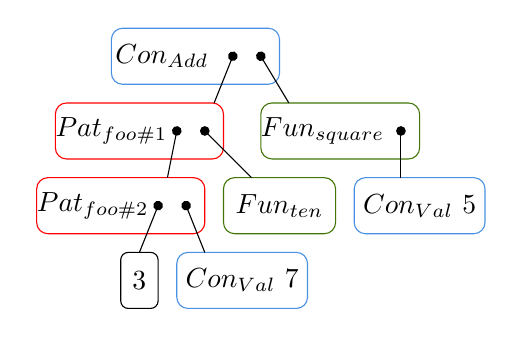
\begin{tikzpicture}[x=0.75pt,y=0.75pt,yscale=-0.9,xscale=0.9]
%uncomment if require: \path (0,440.8571319580078); %set diagram left start at 0, and has height of 440.8571319580078

%Rounded Rect [id:dp48618213158536694]
\draw  [color={rgb, 255:red, 74; green, 144; blue, 226 }  ,draw opacity=1 ] (190,196) .. controls (190,192.69) and (192.69,190) .. (196,190) -- (254,190) .. controls (257.31,190) and (260,192.69) .. (260,196) -- (260,214) .. controls (260,217.31) and (257.31,220) .. (254,220) -- (196,220) .. controls (192.69,220) and (190,217.31) .. (190,214) -- cycle ;

%Rounded Rect [id:dp009025103452140248]
\draw  [color={rgb, 255:red, 74; green, 144; blue, 226 }  ,draw opacity=1 ] (95,236) .. controls (95,232.69) and (97.69,230) .. (101,230) -- (159,230) .. controls (162.31,230) and (165,232.69) .. (165,236) -- (165,254) .. controls (165,257.31) and (162.31,260) .. (159,260) -- (101,260) .. controls (97.69,260) and (95,257.31) .. (95,254) -- cycle ;

%Rounded Rect [id:dp9232511876637792]
\draw  [color={rgb, 255:red, 74; green, 144; blue, 226 }  ,draw opacity=1 ] (60,116) .. controls (60,112.69) and (62.69,110) .. (66,110) -- (144,110) .. controls (147.31,110) and (150,112.69) .. (150,116) -- (150,134) .. controls (150,137.31) and (147.31,140) .. (144,140) -- (66,140) .. controls (62.69,140) and (60,137.31) .. (60,134) -- cycle ;

%Rounded Rect [id:dp10823094494105145]
\draw  [color={rgb, 255:red, 255; green, 0; blue, 0 }  ,draw opacity=1 ] (30,156) .. controls (30,152.69) and (32.69,150) .. (36,150) -- (114,150) .. controls (117.31,150) and (120,152.69) .. (120,156) -- (120,174) .. controls (120,177.31) and (117.31,180) .. (114,180) -- (36,180) .. controls (32.69,180) and (30,177.31) .. (30,174) -- cycle ;

%Rounded Rect [id:dp509725264431323]
\draw  [color={rgb, 255:red, 255; green, 0; blue, 0 }  ,draw opacity=1 ] (20,196) .. controls (20,192.69) and (22.69,190) .. (26,190) -- (104,190) .. controls (107.31,190) and (110,192.69) .. (110,196) -- (110,214) .. controls (110,217.31) and (107.31,220) .. (104,220) -- (26,220) .. controls (22.69,220) and (20,217.31) .. (20,214) -- cycle ;

%Rounded Rect [id:dp3455746100780601]
\draw   (65,234) .. controls (65,231.79) and (66.79,230) .. (69,230) -- (81,230) .. controls (83.21,230) and (85,231.79) .. (85,234) -- (85,256) .. controls (85,258.21) and (83.21,260) .. (81,260) -- (69,260) .. controls (66.79,260) and (65,258.21) .. (65,256) -- cycle ;

%Rounded Rect [id:dp5622973663481885]
\draw  [color={rgb, 255:red, 65; green, 117; blue, 5 }  ,draw opacity=1 ] (140,156) .. controls (140,152.69) and (142.69,150) .. (146,150) -- (219,150) .. controls (222.31,150) and (225,152.69) .. (225,156) -- (225,174) .. controls (225,177.31) and (222.31,180) .. (219,180) -- (146,180) .. controls (142.69,180) and (140,177.31) .. (140,174) -- cycle ;

%Rounded Rect [id:dp33414100410678915]
\draw  [color={rgb, 255:red, 65; green, 117; blue, 5 }  ,draw opacity=1 ] (120,196) .. controls (120,192.69) and (122.69,190) .. (126,190) -- (174,190) .. controls (177.31,190) and (180,192.69) .. (180,196) -- (180,214) .. controls (180,217.31) and (177.31,220) .. (174,220) -- (126,220) .. controls (122.69,220) and (120,217.31) .. (120,214) -- cycle ;

%Straight Lines [id:da7735002123972574]
\draw    (140,125) -- (155,150) ;

\draw [shift={(140,125)}, rotate = 59.04] [color={rgb, 255:red, 0; green, 0; blue, 0 }  ][fill={rgb, 255:red, 0; green, 0; blue, 0 }  ][line width=0.75]      (0, 0) circle [x radius= 2, y radius= 2]   ;
%Straight Lines [id:da19830589256441322]
\draw    (125,125) -- (115,150) ;

\draw [shift={(125,125)}, rotate = 111.8] [color={rgb, 255:red, 0; green, 0; blue, 0 }  ][fill={rgb, 255:red, 0; green, 0; blue, 0 }  ][line width=0.75]      (0, 0) circle [x radius= 2, y radius= 2]   ;
%Straight Lines [id:da7234273703208924]
\draw    (95,165) -- (90,190) ;

\draw [shift={(95,165)}, rotate = 101.31] [color={rgb, 255:red, 0; green, 0; blue, 0 }  ][fill={rgb, 255:red, 0; green, 0; blue, 0 }  ][line width=0.75]      (0, 0) circle [x radius= 2, y radius= 2]   ;
%Straight Lines [id:da39520289035501]
\draw    (110,165) -- (135,190) ;

\draw [shift={(110,165)}, rotate = 45] [color={rgb, 255:red, 0; green, 0; blue, 0 }  ][fill={rgb, 255:red, 0; green, 0; blue, 0 }  ][line width=0.75]      (0, 0) circle [x radius= 2, y radius= 2]   ;
%Straight Lines [id:da4431461097782077]
\draw    (215,165) -- (215,190) ;

\draw [shift={(215,165)}, rotate = 90] [color={rgb, 255:red, 0; green, 0; blue, 0 }  ][fill={rgb, 255:red, 0; green, 0; blue, 0 }  ][line width=0.75]      (0, 0) circle [x radius= 2, y radius= 2]   ;
%Straight Lines [id:da8121818084178258]
\draw    (85,205) -- (75,230) ;

\draw [shift={(85,205)}, rotate = 111.8] [color={rgb, 255:red, 0; green, 0; blue, 0 }  ][fill={rgb, 255:red, 0; green, 0; blue, 0 }  ][line width=0.75]      (0, 0) circle [x radius= 2, y radius= 2]   ;
%Straight Lines [id:da8679389234287274]
\draw    (100,205) -- (110,230) ;

\draw [shift={(100,205)}, rotate = 68.2] [color={rgb, 255:red, 0; green, 0; blue, 0 }  ][fill={rgb, 255:red, 0; green, 0; blue, 0 }  ][line width=0.75]      (0, 0) circle [x radius= 2, y radius= 2]   ;

% Text Node
\draw (225,205) node   {$Con_{Val} \ 5$};
% Text Node
\draw (130,245) node   {$Con_{Val} \ 7$};
% Text Node
\draw (87,125) node   {$Con_{Add}$};
% Text Node
\draw (60,165) node   {$Pat_{foo\#1}$};
% Text Node
\draw (50,205) node   {$Pat_{foo\#2}$};
% Text Node
\draw (75,245) node   {$3$};
% Text Node
\draw (173.05,165) node   {$Fun_{square}$};
% Text Node
\draw (150,205) node   {$Fun_{ten}$};

\end{tikzpicture}

%   \caption{Some caption.}
%   \label{fig:val}
% \end{figure}


We want to remark that, for space reasons, we were only able to introduce the
representation of a rather simple target data type.
%
In practice, this reasoning can be extended to mutually recursive and parametric
types as well.


Overall, this approach offers significant advantages over the usual type-driven
derivation of random generators:
%
\begin{itemize}
\item \textbf{Composability:} we can combine different atomic representations
  using different structure information sources depending on what property or
  sub-system we need to verify using randomly generated values.
  %
\item \textbf{Extensibility:} the developer can derive representations for new
  sources of structure information and combine them with the existing ones
  simply by adding them to the existing generation specification of the target
  data type.
  %
\item \textbf{Predictability:} using branching processes theory, it is possible
  to predict the average distribution of generated values in terms of number of
  constructors.
  %
  This prediction is completely modular, and can be obtained for any composite
  representation obtained using the automatically derived \ensuremath{\Conid{HRep}}s and the
  provided combinators.
\end{itemize}

\todo[author=AM, inline]{Maybe we can show an example random value from the representation
  and its corresponding target value }



% \begin{align*}
%   \llbracket \_ \rrbracket_{target}\ :\ rep_{target}\ \rightarrow\ target
% \end{align*}
%
% \begin{code}
% class (rep down target) where
%   step :: rep target -> target
% \end{code}
%
% \begin{code}
% data (Term f) a = TagTerm (f a)

% \begin{code}
% instance (HRep_Val down Exp) where
%   step (Mk_Val n) = Val n

% instance (HRep_Add down Exp) where
%   step (Mk_Add x y) = Add x y

% instance (HRep_Mul down Exp) where
%   step (Mk_Mul x y) = Mul x y
% \end{code}

% \begin{code}
% instance (f otimes n down Exp) where
%   step (Freq f) = step f
% \end{code}

% \begin{code}
% instance Arbitrary1 (f otimes n) where
%   liftArbitrary gen_HRep = Tag <$> gen_HRep
% \end{code} %$

% instance (Term f down Exp) where
%   step (TagTerm f) = step f
% \end{code}

% \begin{code}
% instance (HRep_ten down Exp) where
%   step Mk_ten = ten

% instance (HRep_square down Exp) where
%   step (Mk_square x) = square x

% instance (HRep_minus down Exp) where
%   step (Mk_minus x y) = minus x y
% \end{code}

% \begin{code}
% instance Arbitrary1 HRep_ten where
%   liftArbitrary gen_HRep = pure Mk_ten

% instance Arbitrary1 HRep_square where
%   liftArbitrary gen_HRep = Mk_square <$> gen_HRep

% instance Arbitrary1 HRep_minus where
%   liftArbitrary gen_HRep
%     = Mk_minus <$> gen_HRep <*> gen_HRep
% \end{code} %$

% \begin{code}
% instance (HRep_foo_1 down Exp) where
%   step (Mk_foo_1 x y)
%     = Add (Add x (Val 50)) (Add (Val 25) y)

% instance (HRep_foo_2 down Exp) where
%   step (Mk_foo_2 x y)
%     = Mul (Val 50) (Mul (Val x) y)
% \end{code}

% \begin{code}
% instance Arbitrary1 HRep_foo_1 where
%   liftArbitrary gen_HRep
%     = Mk_foo_1 <$> gen_HRep <*> gen_HRep

% instance Arbitrary1 HRep_foo_2 where
%   liftArbitrary gen_HRep
%     = Mk_foo_2 <$> arbitrary <*> gen_HRep
% \end{code} %$

% \begin{code}
% instance (f oplus g down Exp) where
%   step (L f) = step f
%   step (R g) = step g
% \end{code}

% \begin{code}
% instance Arbitrary1 (f oplus g) where
%   liftArbitrary gen_HRep
%     = frequency
%       [ (freq at_f, L <$> gen_HRep)
%       , (freq at_g, R <$> gen_HRep) ]
% \end{code} %$

% \begin{figure}[b]
%   \centering
%   
\tikzset{every picture/.style={line width=0.75pt}} %set default line width to 0.75pt

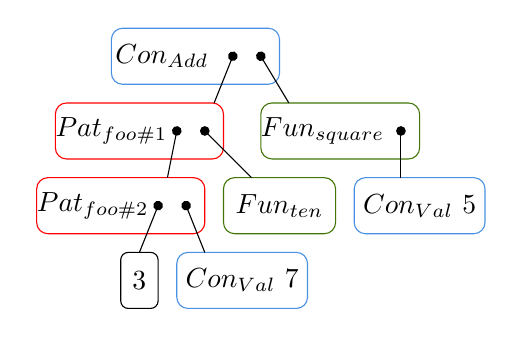
\begin{tikzpicture}[x=0.75pt,y=0.75pt,yscale=-0.9,xscale=0.9]
%uncomment if require: \path (0,440.8571319580078); %set diagram left start at 0, and has height of 440.8571319580078

%Rounded Rect [id:dp48618213158536694]
\draw  [color={rgb, 255:red, 74; green, 144; blue, 226 }  ,draw opacity=1 ] (190,196) .. controls (190,192.69) and (192.69,190) .. (196,190) -- (254,190) .. controls (257.31,190) and (260,192.69) .. (260,196) -- (260,214) .. controls (260,217.31) and (257.31,220) .. (254,220) -- (196,220) .. controls (192.69,220) and (190,217.31) .. (190,214) -- cycle ;

%Rounded Rect [id:dp009025103452140248]
\draw  [color={rgb, 255:red, 74; green, 144; blue, 226 }  ,draw opacity=1 ] (95,236) .. controls (95,232.69) and (97.69,230) .. (101,230) -- (159,230) .. controls (162.31,230) and (165,232.69) .. (165,236) -- (165,254) .. controls (165,257.31) and (162.31,260) .. (159,260) -- (101,260) .. controls (97.69,260) and (95,257.31) .. (95,254) -- cycle ;

%Rounded Rect [id:dp9232511876637792]
\draw  [color={rgb, 255:red, 74; green, 144; blue, 226 }  ,draw opacity=1 ] (60,116) .. controls (60,112.69) and (62.69,110) .. (66,110) -- (144,110) .. controls (147.31,110) and (150,112.69) .. (150,116) -- (150,134) .. controls (150,137.31) and (147.31,140) .. (144,140) -- (66,140) .. controls (62.69,140) and (60,137.31) .. (60,134) -- cycle ;

%Rounded Rect [id:dp10823094494105145]
\draw  [color={rgb, 255:red, 255; green, 0; blue, 0 }  ,draw opacity=1 ] (30,156) .. controls (30,152.69) and (32.69,150) .. (36,150) -- (114,150) .. controls (117.31,150) and (120,152.69) .. (120,156) -- (120,174) .. controls (120,177.31) and (117.31,180) .. (114,180) -- (36,180) .. controls (32.69,180) and (30,177.31) .. (30,174) -- cycle ;

%Rounded Rect [id:dp509725264431323]
\draw  [color={rgb, 255:red, 255; green, 0; blue, 0 }  ,draw opacity=1 ] (20,196) .. controls (20,192.69) and (22.69,190) .. (26,190) -- (104,190) .. controls (107.31,190) and (110,192.69) .. (110,196) -- (110,214) .. controls (110,217.31) and (107.31,220) .. (104,220) -- (26,220) .. controls (22.69,220) and (20,217.31) .. (20,214) -- cycle ;

%Rounded Rect [id:dp3455746100780601]
\draw   (65,234) .. controls (65,231.79) and (66.79,230) .. (69,230) -- (81,230) .. controls (83.21,230) and (85,231.79) .. (85,234) -- (85,256) .. controls (85,258.21) and (83.21,260) .. (81,260) -- (69,260) .. controls (66.79,260) and (65,258.21) .. (65,256) -- cycle ;

%Rounded Rect [id:dp5622973663481885]
\draw  [color={rgb, 255:red, 65; green, 117; blue, 5 }  ,draw opacity=1 ] (140,156) .. controls (140,152.69) and (142.69,150) .. (146,150) -- (219,150) .. controls (222.31,150) and (225,152.69) .. (225,156) -- (225,174) .. controls (225,177.31) and (222.31,180) .. (219,180) -- (146,180) .. controls (142.69,180) and (140,177.31) .. (140,174) -- cycle ;

%Rounded Rect [id:dp33414100410678915]
\draw  [color={rgb, 255:red, 65; green, 117; blue, 5 }  ,draw opacity=1 ] (120,196) .. controls (120,192.69) and (122.69,190) .. (126,190) -- (174,190) .. controls (177.31,190) and (180,192.69) .. (180,196) -- (180,214) .. controls (180,217.31) and (177.31,220) .. (174,220) -- (126,220) .. controls (122.69,220) and (120,217.31) .. (120,214) -- cycle ;

%Straight Lines [id:da7735002123972574]
\draw    (140,125) -- (155,150) ;

\draw [shift={(140,125)}, rotate = 59.04] [color={rgb, 255:red, 0; green, 0; blue, 0 }  ][fill={rgb, 255:red, 0; green, 0; blue, 0 }  ][line width=0.75]      (0, 0) circle [x radius= 2, y radius= 2]   ;
%Straight Lines [id:da19830589256441322]
\draw    (125,125) -- (115,150) ;

\draw [shift={(125,125)}, rotate = 111.8] [color={rgb, 255:red, 0; green, 0; blue, 0 }  ][fill={rgb, 255:red, 0; green, 0; blue, 0 }  ][line width=0.75]      (0, 0) circle [x radius= 2, y radius= 2]   ;
%Straight Lines [id:da7234273703208924]
\draw    (95,165) -- (90,190) ;

\draw [shift={(95,165)}, rotate = 101.31] [color={rgb, 255:red, 0; green, 0; blue, 0 }  ][fill={rgb, 255:red, 0; green, 0; blue, 0 }  ][line width=0.75]      (0, 0) circle [x radius= 2, y radius= 2]   ;
%Straight Lines [id:da39520289035501]
\draw    (110,165) -- (135,190) ;

\draw [shift={(110,165)}, rotate = 45] [color={rgb, 255:red, 0; green, 0; blue, 0 }  ][fill={rgb, 255:red, 0; green, 0; blue, 0 }  ][line width=0.75]      (0, 0) circle [x radius= 2, y radius= 2]   ;
%Straight Lines [id:da4431461097782077]
\draw    (215,165) -- (215,190) ;

\draw [shift={(215,165)}, rotate = 90] [color={rgb, 255:red, 0; green, 0; blue, 0 }  ][fill={rgb, 255:red, 0; green, 0; blue, 0 }  ][line width=0.75]      (0, 0) circle [x radius= 2, y radius= 2]   ;
%Straight Lines [id:da8121818084178258]
\draw    (85,205) -- (75,230) ;

\draw [shift={(85,205)}, rotate = 111.8] [color={rgb, 255:red, 0; green, 0; blue, 0 }  ][fill={rgb, 255:red, 0; green, 0; blue, 0 }  ][line width=0.75]      (0, 0) circle [x radius= 2, y radius= 2]   ;
%Straight Lines [id:da8679389234287274]
\draw    (100,205) -- (110,230) ;

\draw [shift={(100,205)}, rotate = 68.2] [color={rgb, 255:red, 0; green, 0; blue, 0 }  ][fill={rgb, 255:red, 0; green, 0; blue, 0 }  ][line width=0.75]      (0, 0) circle [x radius= 2, y radius= 2]   ;

% Text Node
\draw (225,205) node   {$Con_{Val} \ 5$};
% Text Node
\draw (130,245) node   {$Con_{Val} \ 7$};
% Text Node
\draw (87,125) node   {$Con_{Add}$};
% Text Node
\draw (60,165) node   {$Pat_{foo\#1}$};
% Text Node
\draw (50,205) node   {$Pat_{foo\#2}$};
% Text Node
\draw (75,245) node   {$3$};
% Text Node
\draw (173.05,165) node   {$Fun_{square}$};
% Text Node
\draw (150,205) node   {$Fun_{ten}$};

\end{tikzpicture}

%   \caption{Higher level representation of the data type |Exp|, defined using
%     structural information from the function |foo| and the abstract interface of
%     the module |M|.}
%   \label{fig:hrep}
% \end{figure}

\newpage

\section{Random Generators Synthesis} \label{sec:synthesis}

Aliquam erat volutpat. Nunc eleifend leo vitae magna. In id erat non orci
commodo lobortis. Proin neque massa, cursus ut, gravida ut, lobortis eget,
lacus. Sed diam. Praesent fermentum tempor tellus. Nullam tempus. Mauris ac
felis vel velit tristique imperdiet. Donec at pede. Etiam vel neque nec dui
dignissim bibendum. Vivamus id enim. Phasellus neque orci, porta a, aliquet
quis, semper a, massa. Phasellus purus. Pellentesque tristique imperdiet tortor.
Nam euismod tellus id erat.

\newpage

\section{Case Studies}

Aliquam erat volutpat. Nunc eleifend leo vitae magna. In id erat non orci
commodo lobortis. Proin neque massa, cursus ut, gravida ut, lobortis eget,
lacus. Sed diam. Praesent fermentum tempor tellus. Nullam tempus. Mauris ac
felis vel velit tristique imperdiet. Donec at pede. Etiam vel neque nec dui
dignissim bibendum. Vivamus id enim. Phasellus neque orci, porta a, aliquet
quis, semper a, massa. Phasellus purus. Pellentesque tristique imperdiet tortor.
Nam euismod tellus id erat.

\begin{figure}[t]
  \centering
  \pgfplotsset{scaled y ticks=false}
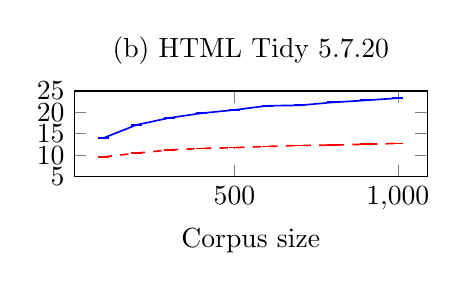
\begin{tikzpicture}
  \begin{axis}[
    title={(b) HTML Tidy 5.7.20},
    height=0.22\textwidth,
    width=0.5\textwidth,
    xlabel={Corpus size},
    % ylabel={Different execution paths (thousands)},
    % y tick label style={rotate=45,anchor=east},
    % ymajorgrids=true,
    legend pos=south east,
    legend cell align={left},
    % xmin=100, xmax=1000,
    ymin=5, ymax=25,
    enlarge x limits=0.1
    % enlarge y limits=0.1
    ]
    \addplot+[blue][semithick, mark=none,
    error bars/.cd, y dir=both, y explicit]
    coordinates {
      (100,  14.01417) +- (0.0, 0.14883523)
      (200,  17.05810) +- (0.0, 0.13506726)
      (300,  18.68763) +- (0.0, 0.11803936)
      (400,  19.80227) +- (0.0, 0.15292292)
      (500,  20.55840) +- (0.0, 0.13536179)
      (600,  21.53490) +- (0.0, 0.10085658)
      (700,  21.63750) +- (0.0, 0.10470160)
      (800,  22.32833) +- (0.0, 0.11168286)
      (900,  22.78813) +- (0.0, 0.10231978)
      (1000, 23.32330) +- (0.0, 0.09762431)
    };
    \label{exp:dragenp}
    % \addlegendentry{\dragenp};
    % \addplot+[blue][semithick, mark=none,
    % error bars/.cd, y dir=both, y explicit]
    % coordinates {
    %   (100,  12805.40) +- (0.0, 234.61546)
    %   (200,  15382.40) +- (0.0, 172.25118)
    %   (300,  16984.87) +- (0.0, 106.89291)
    %   (400,  17695.77) +- (0.0, 157.54098)
    %   (500,  18670.37) +- (0.0, 138.47555)
    %   (600,  19197.10) +- (0.0, 137.48348)
    %   (700,  19934.90) +- (0.0, 97.24403 )
    %   (800,  20430.27) +- (0.0, 129.08726)
    %   (900,  20775.97) +- (0.0, 136.66240)
    %   (1000, 21264.20) +- (0.0, 102.07806)
    % };
    % \addlegendentry{\dragenp};
    \addplot+[red][semithick, dashed, mark=none,
    error bars/.cd, y dir=both, y explicit,
    error bar style={solid}
    ]
    coordinates {
      (100,  09.574067) +- (0.0, 0.05736926)
      (200,  10.451433) +- (0.0, 0.04399278)
      (300,  11.195367) +- (0.0, 0.03931592)
      (400,  11.556767) +- (0.0, 0.04036912)
      (500,  11.738333) +- (0.0, 0.04965803)
      (600,  12.028333) +- (0.0, 0.04250789)
      (700,  12.257100) +- (0.0, 0.03936573)
      (800,  12.334567) +- (0.0, 0.04082921)
      (900,  12.536733) +- (0.0, 0.04470660)
      (1000, 12.731967) +- (0.0, 0.04069840)
    };
    \label{exp:dragen}
    % \addlegendentry{\dragen};
  \end{axis}
\end{tikzpicture}
  \caption{Something something.}
  \label{fig:html}
\end{figure}

Aliquam erat volutpat. Nunc eleifend leo vitae magna. In id erat non orci
commodo lobortis. Proin neque massa, cursus ut, gravida ut, lobortis eget,
lacus. Sed diam. Praesent fermentum tempor tellus. Nullam tempus. Mauris ac
felis vel velit tristique imperdiet. Donec at pede. Etiam vel neque nec dui
dignissim bibendum. Vivamus id enim. Phasellus neque orci, porta a, aliquet
quis, semper a, massa. Phasellus purus. Pellentesque tristique imperdiet tortor.
Nam euismod tellus id erat.

Lorem ipsum dolor sit amet, consectetuer adipiscing elit. Donec hendrerit tempor
tellus. Donec pretium posuere tellus. Proin quam nisl, tincidunt et, mattis
eget, convallis nec, purus. Cum sociis natoque penatibus et magnis dis
parturient montes, nascetur ridiculus mus. Nulla posuere. Donec vitae dolor.
Nullam tristique diam non turpis. Cras placerat accumsan nulla. Nullam rutrum.
Nam vestibulum accumsan nisl.

Nullam eu ante vel est convallis dignissim. Fusce suscipit, wisi nec facilisis
facilisis, est dui fermentum leo, quis tempor ligula erat quis odio. Nunc porta
vulputate tellus. Nunc rutrum turpis sed pede. Sed bibendum. Aliquam posuere.
Nunc aliquet, augue nec adipiscing interdum, lacus tellus malesuada massa, quis
varius mi purus non odio. Pellentesque condimentum, magna ut suscipit hendrerit,
ipsum augue ornare nulla, non luctus diam neque sit amet urna. Curabitur
vulputate vestibulum lorem. Fusce sagittis, libero non molestie mollis, magna
orci ultrices dolor, at vulputate neque nulla lacinia eros. Sed id ligula quis
est convallis tempor. Curabitur lacinia pulvinar nibh. Nam a sapien.

\newpage

\section{Related Work}

Aliquam erat volutpat. Nunc eleifend leo vitae magna. In id erat non orci
commodo lobortis. Proin neque massa, cursus ut, gravida ut, lobortis eget,
lacus. Sed diam. Praesent fermentum tempor tellus. Nullam tempus. Mauris ac
felis vel velit tristique imperdiet. Donec at pede. Etiam vel neque nec dui
dignissim bibendum. Vivamus id enim. Phasellus neque orci, porta a, aliquet
quis, semper a, massa. Phasellus purus. Pellentesque tristique imperdiet tortor.
Nam euismod tellus id erat.

\newpage

\section{Final Remarks}

Nullam eu ante vel est convallis dignissim. Fusce suscipit, wisi nec facilisis
facilisis, est dui fermentum leo, quis tempor ligula erat quis odio. Nunc porta
vulputate tellus. Nunc rutrum turpis sed pede. Sed bibendum. Aliquam posuere.
Nunc aliquet, augue nec adipiscing interdum, lacus tellus malesuada massa, quis
varius mi purus non odio. Pellentesque condimentum, magna ut suscipit hendrerit,
ipsum augue ornare nulla, non luctus diam neque sit amet urna. Curabitur
vulputate vestibulum lorem.

%%%%%%%%%%%%%%%%%%%%%%%%%%%%%%%%%%%%%%%%
%% Bibliography
\bibliographystyle{IEEEtran}
\bibliography{references.bib}

\end{document}
